% lecture7_ro.tex -- GENERATED by build_L7.py from L7_numbers.json; do not edit by hand.
\documentclass[10pt,aspectratio=169,t]{beamer}
% =============================================================================
% emqa_preamble.tex -- shared Beamer preamble of Energy Markets Quantitative Analysis (EMQA)
% Used by every lecture: lectures/Lk/lecturek.tex does
%   \documentclass[10pt,aspectratio=169,t]{beamer}
%   % =============================================================================
% emqa_preamble.tex -- shared Beamer preamble of Energy Markets Quantitative Analysis (EMQA)
% Used by every lecture: lectures/Lk/lecturek.tex does
%   \documentclass[10pt,aspectratio=169,t]{beamer}
%   % =============================================================================
% emqa_preamble.tex -- shared Beamer preamble of Energy Markets Quantitative Analysis (EMQA)
% Used by every lecture: lectures/Lk/lecturek.tex does
%   \documentclass[10pt,aspectratio=169,t]{beamer}
%   \input{../common/emqa_preamble}
%   \emqalecture{k}{Lecture title}
% Logos live in lectures/common/logos/, charts in lectures/Lk/charts/.
% Do NOT add \hfuzz / \vfuzz / \hbadness here: overfull boxes must be fixed, not hidden.
% =============================================================================

\usetheme{default}
\setbeamersize{text margin left=7mm, text margin right=7mm}

% ---------------------------------------------------------------- packages
\usepackage[utf8]{inputenc}
\usepackage[T1]{fontenc}
\usepackage{lmodern}
\usepackage{amsmath, amssymb}
\usepackage{mathtools}
\usepackage{bm}
\usepackage{tikz}
\usetikzlibrary{arrows.meta, positioning, calc, shapes.misc}
\usepackage{booktabs}
\usepackage{array}
\usepackage{graphicx}
\usepackage{colortbl}
\usepackage{xcolor}
\usepackage{multicol}
\hypersetup{colorlinks=true, linkcolor=MainBlue, urlcolor=MainBlue, citecolor=MainBlue}
\graphicspath{{../common/logos/}}   % charts are included with their language folder: charts/en/, charts/ro/

% ---------------------------------------------------------------- colours
\definecolor{MainBlue}{RGB}{26, 58, 110}
\definecolor{IDAred}{RGB}{205, 0, 0}
\definecolor{DarkGray}{RGB}{51, 51, 51}
\definecolor{FooterGray}{RGB}{100, 100, 100}
\definecolor{BlockGray}{RGB}{236, 238, 242}
\definecolor{KeynoteGray}{RGB}{218, 218, 218}
\definecolor{Crimson}{RGB}{190, 40, 50}
\definecolor{Forest}{RGB}{30, 110, 50}
\definecolor{Bitter}{RGB}{214, 150, 20}
% chart palette (same hex values as lectures/common/emqa_plot.py)
\definecolor{SerRO}{HTML}{2A78D6}
\definecolor{SerDE}{HTML}{EB6834}
\definecolor{SerHU}{HTML}{1BAF7A}
\definecolor{SerBG}{HTML}{EDA100}

\setbeamertemplate{background}{%
  \begin{tikzpicture}[remember picture, overlay]
    \shade[shading=axis, shading angle=315, top color=white, bottom color=KeynoteGray]
      (current page.south west) rectangle (current page.north east);
  \end{tikzpicture}}
\setbeamercolor{background canvas}{bg=}
\setbeamercolor{structure}{fg=MainBlue}
\setbeamercolor{normal text}{fg=DarkGray}
\setbeamercolor{title}{fg=IDAred}
\setbeamercolor{frametitle}{fg=IDAred, bg=}
\setbeamercolor{block title}{bg=MainBlue, fg=white}
\setbeamercolor{block body}{bg=BlockGray, fg=DarkGray}
\setbeamercolor{block title alerted}{bg=Crimson, fg=white}
\setbeamercolor{block body alerted}{bg=Crimson!7, fg=DarkGray}
\setbeamercolor{block title example}{bg=Forest, fg=white}
\setbeamercolor{block body example}{bg=Forest!7, fg=DarkGray}
\setbeamercolor{item}{fg=MainBlue}
\setbeamerfont{frametitle}{size=\large, series=\bfseries}
\setbeamerfont{block title}{size=\small, series=\bfseries}
\setbeamertemplate{blocks}[rounded][shadow=false]
\setbeamertemplate{itemize item}{\color{MainBlue}$\boxdot$}
\setbeamertemplate{itemize subitem}{\color{MainBlue}\scriptsize$\blacktriangleright$}
% compact two-level lists: level 1 = main point, level 2 = details (no text outside bullets)
\setbeamerfont{itemize/enumerate subbody}{size=\footnotesize}
\setlength{\leftmargini}{1.1em}
\setlength{\leftmarginii}{1.1em}
\setbeamertemplate{itemize/enumerate body begin}{\setlength{\topsep}{0pt}\setlength{\partopsep}{0pt}\setlength{\parskip}{0pt}}
\setbeamertemplate{itemize/enumerate subbody begin}{\setlength{\topsep}{0pt}\setlength{\partopsep}{0pt}\setlength{\itemsep}{0pt}\vspace{-0.4ex}}

\setbeamertemplate{enumerate item}{\color{MainBlue}\insertenumlabel.}
\setlength{\leftmargini}{1.3em}
\setlength{\leftmarginii}{1.2em}
\setbeamertemplate{navigation symbols}{}
\setbeamertemplate{section in toc}{\color{MainBlue}$\blacktriangleright$~\inserttocsection}
\setbeamertemplate{caption}{\raggedright\insertcaption\par}
% frame subtitle = precise citation line under the claim title (Weron style)
\setbeamerfont{framesubtitle}{size=\footnotesize}
\setbeamercolor{framesubtitle}{fg=FooterGray}
% outline that reappears at every section with the current section highlighted
\setbeamertemplate{section in toc shaded}[default][35]
\setbeamertemplate{subsection in toc shaded}[default][35]
\setbeamertemplate{subsection in toc}{\leavevmode\leftskip=2.2em\color{DarkGray}\small\inserttocsubsection\par}
\AtBeginSection[]{{\begin{frame}{\txtoutline}\vspace{2mm}\small
  \tableofcontents[currentsection,hideothersubsections]\end{frame}}}

% ---------------------------------------------------------------- head and foot
\setbeamertemplate{headline}{%
  \vskip10pt%
  \hbox to \paperwidth{\hskip0.5cm%
    {\small\color{FooterGray}\renewcommand{\hyperlink}[2]{##2}\insertsectionhead}%
    \hfill\textcolor{FooterGray}{\small\insertframenumber}\hskip0.5cm}%
  \vskip4pt{\color{FooterGray}\hrule height 0.4pt}}
% footer as in the other courses (MFM, SFM): course name on the left, small sparkline on the right
\setbeamertemplate{footline}{%
  {\color{FooterGray}\hrule height 0.4pt}\vskip4pt%
  \hbox to \paperwidth{\hskip0.5cm%
    \textcolor{FooterGray}{\small\txtcourse}%
    \hfill\raisebox{-0.1em}{\begin{tikzpicture}[x=0.08em, y=0.08em, line width=0.4pt]
      \draw[FooterGray] (0,3) -- (1,4) -- (2,3.5) -- (3,5) -- (4,4) -- (5,6) -- (6,5.5) -- (7,4) -- (8,5) -- (9,7) -- (10,6) -- (11,5) -- (12,6.5) -- (13,8) -- (14,7) -- (15,6) -- (16,7.5) -- (17,9) -- (18,8) -- (19,7) -- (20,8.5) -- (21,10) -- (22,9) -- (23,8) -- (24,9.5);
    \end{tikzpicture}}\hskip0.5cm}%
  \vskip6pt}

% ---------------------------------------------------------------- title page
\defbeamertemplate*{title page}{emqa}[1][]{%
  \vspace{0.15cm}
  \begin{center}
    \href{https://www.ase.ro}{
\includegraphics[height=0.9cm]{ase_logo.png}}\hspace{0.3cm}%
    \href{https://ipe.ro/new}{
\includegraphics[height=0.9cm]{acad_logo.png}}\hspace{0.3cm}%
    \href{https://theida.net}{
\includegraphics[height=0.9cm]{ida_logo.png}}\hspace{0.3cm}%
    \href{https://blockchain-research-center.com}{
\includegraphics[height=0.9cm]{brc_logo.png}}\hspace{0.3cm}%
    \href{https://www.ai4efin.ase.ro}{
\includegraphics[height=0.9cm]{ai4efin_logo.png}}\hspace{0.3cm}%
    \href{https://www.digital-finance-msca.com}{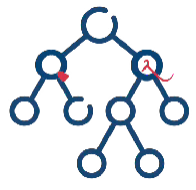
\includegraphics[height=0.9cm]{msca_logo.png}}%
  \end{center}
  \vspace{0.45cm}
  \begin{center}
    \begin{minipage}{0.1\textwidth}\centering
      \href{https://quantlet.com}{
\includegraphics[height=0.9cm]{ql_logo.png}}\end{minipage}%
    \begin{minipage}{0.78\textwidth}\centering
      {\Large\bfseries\usebeamercolor[fg]{title}\inserttitle}\par\vspace{0.25cm}
      {\large\usebeamercolor[fg]{title}\insertsubtitle}\end{minipage}%
    \begin{minipage}{0.1\textwidth}\centering
      \href{https://quantinar.com}{
\includegraphics[height=0.9cm]{qr_logo.png}}\end{minipage}
  \end{center}
  \vfill
  \hspace{0.4cm}{\bfseries\insertauthor}\par\vspace{0.12cm}
  \hspace{0.4cm}\begin{minipage}[t]{0.92\textwidth}\raggedright\footnotesize\insertinstitute\end{minipage}
  \par\vspace{0.4cm}}

% ---------------------------------------------------------------- lecture metadata
\newcommand{\emqashort}{}
\newcommand{\emqanb}{notebooks}
\newcommand{\emqarepo}{https://github.com/danpele/EMQA/tree/main}
% language-dependent labels (English default; \emqaromanian switches to Romanian, call it before \emqalecture)
\newcommand{\txtcourse}{Energy Markets Quantitative Analysis}
\newcommand{\txtlecture}{Lecture}
\newcommand{\txtoutline}{Outline}
\newcommand{\txtintuition}{In one sentence:}
\newcommand{\txtjob}{In practice:}
\newcommand{\txttry}{Experiment yourself:}
\newcommand{\txtwhere}{where}
\newcommand{\txtsim}{SIMULATED DATA (teaching illustration)}
\newcommand{\txtnbsuffix}{}
\newcommand{\txtinstitute}{Bucharest University of Economic Studies, Department of Statistics and Econometrics\\
    Romanian Academy, Institute for Economic Forecasting\\
    IDA Institute Digital Assets \textbullet\ AI4EFin \textbullet\ MSCA Digital Finance}
\newcommand{\emqaromanian}{%
  \renewcommand{\txtcourse}{Analiza cantitativă a piețelor de energie}%
  \renewcommand{\txtlecture}{Cursul}%
  \renewcommand{\txtoutline}{Cuprins}%
  \renewcommand{\txtintuition}{Pe scurt:}%
  \renewcommand{\txtjob}{În practică:}%
  \renewcommand{\txttry}{Exercițiu practic:}%
  \renewcommand{\txtwhere}{unde}%
  \renewcommand{\txtsim}{DATE SIMULATE (doar pentru ilustrare)}%
  \renewcommand{\txtnbsuffix}{\string_ro}%
  \renewcommand{\txtinstitute}{Academia de Studii Economice din București, Departamentul de Statistică și Econometrie\\
    Academia Română, Institutul de Prognoză Economică\\
    IDA Institute Digital Assets \textbullet\ AI4EFin \textbullet\ MSCA Digital Finance}}
\newcommand{\emqalecture}[2]{%
  \renewcommand{\emqashort}{\txtlecture\ #1}%
  \renewcommand{\emqanb}{notebooks/L#1\string_notebook\txtnbsuffix.ipynb}%
  \title[EMQA]{\txtcourse}%
  \subtitle{\txtlecture\ #1: #2}%
  \author{Prof.\ dr.\ Daniel Traian PELE}%
  \institute{\txtinstitute}%
  \date{}}

% ---------------------------------------------------------------- teaching blocks (MBA clarity rule)
% \intuition{one plain sentence}  ->  formula with every symbol defined  ->  real-data example  ->  \manager{one line}
\newcommand{\intuition}[1]{\begin{itemize}\item {\color{MainBlue}\textbf{\txtintuition}}~#1\end{itemize}\vspace{0.6mm}}
\newcommand{\manager}[1]{\colorbox{Forest!10}{\parbox{\dimexpr\linewidth-2\fboxsep\relax}{\footnotesize
  \begin{itemize}\setlength{\itemsep}{0pt}\item \textbf{\color{Forest}\txtjob}~#1\end{itemize}}}}
% Experiment yourself: pointer to the matching notebook section
\newcommand{\tryit}[1]{{\scriptsize\href{\emqarepo/\emqanb}{%
  \raisebox{-0.15em}{
\includegraphics[height=0.85em]{ql_logo.png}}\,\textbf{\txttry}~\color{MainBlue}#1}}}
% bottom row: manager line (left) + experiment pointer (right), pinned to the bottom of the frame
\newcommand{\bottomrow}[2]{\par\vfill\noindent\begin{minipage}[b]{0.72\linewidth}#1\end{minipage}\hfill
  \begin{minipage}[b]{0.26\linewidth}\raggedleft #2\end{minipage}\par\vspace{0.5mm}}
\newcommand{\where}[1]{{\footnotesize\textbf{\txtwhere}~#1\par}}

% ---------------------------------------------------------------- helpers
% chart source line under a figure: \chartsource{Source ...; period ...}
\newcommand{\chartsource}[1]{\par\vspace{1pt}{\scriptsize\color{FooterGray}#1\par}}
% link to code: \quantlet{label}{path inside the repo}
\newcommand{\quantlet}[2]{\par\vspace{1pt}\hfill\href{\emqarepo/#2}{%
  \raisebox{-0.15em}{
\includegraphics[height=0.75em]{ql_logo.png}}\textcolor{MainBlue}{\scriptsize\ #1}}}
\newcommand{\simlabel}{\colorbox{Crimson!12}{\scriptsize\bfseries\color{Crimson}\txtsim}}
\newcommand{\E}{\mathbb{E}}
\newcommand{\Var}{\operatorname{Var}}
\newcommand{\Cov}{\operatorname{Cov}}
\newcommand{\Corr}{\operatorname{Corr}}
\newcommand{\asinh}{\operatorname{asinh}}
\newcommand{\iid}{\overset{\text{i.i.d.}}{\sim}}
\newcommand{\EUR}{EUR}

%   \emqalecture{k}{Lecture title}
% Logos live in lectures/common/logos/, charts in lectures/Lk/charts/.
% Do NOT add \hfuzz / \vfuzz / \hbadness here: overfull boxes must be fixed, not hidden.
% =============================================================================

\usetheme{default}
\setbeamersize{text margin left=7mm, text margin right=7mm}

% ---------------------------------------------------------------- packages
\usepackage[utf8]{inputenc}
\usepackage[T1]{fontenc}
\usepackage{lmodern}
\usepackage{amsmath, amssymb}
\usepackage{mathtools}
\usepackage{bm}
\usepackage{tikz}
\usetikzlibrary{arrows.meta, positioning, calc, shapes.misc}
\usepackage{booktabs}
\usepackage{array}
\usepackage{graphicx}
\usepackage{colortbl}
\usepackage{xcolor}
\usepackage{multicol}
\hypersetup{colorlinks=true, linkcolor=MainBlue, urlcolor=MainBlue, citecolor=MainBlue}
\graphicspath{{../common/logos/}}   % charts are included with their language folder: charts/en/, charts/ro/

% ---------------------------------------------------------------- colours
\definecolor{MainBlue}{RGB}{26, 58, 110}
\definecolor{IDAred}{RGB}{205, 0, 0}
\definecolor{DarkGray}{RGB}{51, 51, 51}
\definecolor{FooterGray}{RGB}{100, 100, 100}
\definecolor{BlockGray}{RGB}{236, 238, 242}
\definecolor{KeynoteGray}{RGB}{218, 218, 218}
\definecolor{Crimson}{RGB}{190, 40, 50}
\definecolor{Forest}{RGB}{30, 110, 50}
\definecolor{Bitter}{RGB}{214, 150, 20}
% chart palette (same hex values as lectures/common/emqa_plot.py)
\definecolor{SerRO}{HTML}{2A78D6}
\definecolor{SerDE}{HTML}{EB6834}
\definecolor{SerHU}{HTML}{1BAF7A}
\definecolor{SerBG}{HTML}{EDA100}

\setbeamertemplate{background}{%
  \begin{tikzpicture}[remember picture, overlay]
    \shade[shading=axis, shading angle=315, top color=white, bottom color=KeynoteGray]
      (current page.south west) rectangle (current page.north east);
  \end{tikzpicture}}
\setbeamercolor{background canvas}{bg=}
\setbeamercolor{structure}{fg=MainBlue}
\setbeamercolor{normal text}{fg=DarkGray}
\setbeamercolor{title}{fg=IDAred}
\setbeamercolor{frametitle}{fg=IDAred, bg=}
\setbeamercolor{block title}{bg=MainBlue, fg=white}
\setbeamercolor{block body}{bg=BlockGray, fg=DarkGray}
\setbeamercolor{block title alerted}{bg=Crimson, fg=white}
\setbeamercolor{block body alerted}{bg=Crimson!7, fg=DarkGray}
\setbeamercolor{block title example}{bg=Forest, fg=white}
\setbeamercolor{block body example}{bg=Forest!7, fg=DarkGray}
\setbeamercolor{item}{fg=MainBlue}
\setbeamerfont{frametitle}{size=\large, series=\bfseries}
\setbeamerfont{block title}{size=\small, series=\bfseries}
\setbeamertemplate{blocks}[rounded][shadow=false]
\setbeamertemplate{itemize item}{\color{MainBlue}$\boxdot$}
\setbeamertemplate{itemize subitem}{\color{MainBlue}\scriptsize$\blacktriangleright$}
% compact two-level lists: level 1 = main point, level 2 = details (no text outside bullets)
\setbeamerfont{itemize/enumerate subbody}{size=\footnotesize}
\setlength{\leftmargini}{1.1em}
\setlength{\leftmarginii}{1.1em}
\setbeamertemplate{itemize/enumerate body begin}{\setlength{\topsep}{0pt}\setlength{\partopsep}{0pt}\setlength{\parskip}{0pt}}
\setbeamertemplate{itemize/enumerate subbody begin}{\setlength{\topsep}{0pt}\setlength{\partopsep}{0pt}\setlength{\itemsep}{0pt}\vspace{-0.4ex}}

\setbeamertemplate{enumerate item}{\color{MainBlue}\insertenumlabel.}
\setlength{\leftmargini}{1.3em}
\setlength{\leftmarginii}{1.2em}
\setbeamertemplate{navigation symbols}{}
\setbeamertemplate{section in toc}{\color{MainBlue}$\blacktriangleright$~\inserttocsection}
\setbeamertemplate{caption}{\raggedright\insertcaption\par}
% frame subtitle = precise citation line under the claim title (Weron style)
\setbeamerfont{framesubtitle}{size=\footnotesize}
\setbeamercolor{framesubtitle}{fg=FooterGray}
% outline that reappears at every section with the current section highlighted
\setbeamertemplate{section in toc shaded}[default][35]
\setbeamertemplate{subsection in toc shaded}[default][35]
\setbeamertemplate{subsection in toc}{\leavevmode\leftskip=2.2em\color{DarkGray}\small\inserttocsubsection\par}
\AtBeginSection[]{{\begin{frame}{\txtoutline}\vspace{2mm}\small
  \tableofcontents[currentsection,hideothersubsections]\end{frame}}}

% ---------------------------------------------------------------- head and foot
\setbeamertemplate{headline}{%
  \vskip10pt%
  \hbox to \paperwidth{\hskip0.5cm%
    {\small\color{FooterGray}\renewcommand{\hyperlink}[2]{##2}\insertsectionhead}%
    \hfill\textcolor{FooterGray}{\small\insertframenumber}\hskip0.5cm}%
  \vskip4pt{\color{FooterGray}\hrule height 0.4pt}}
% footer as in the other courses (MFM, SFM): course name on the left, small sparkline on the right
\setbeamertemplate{footline}{%
  {\color{FooterGray}\hrule height 0.4pt}\vskip4pt%
  \hbox to \paperwidth{\hskip0.5cm%
    \textcolor{FooterGray}{\small\txtcourse}%
    \hfill\raisebox{-0.1em}{\begin{tikzpicture}[x=0.08em, y=0.08em, line width=0.4pt]
      \draw[FooterGray] (0,3) -- (1,4) -- (2,3.5) -- (3,5) -- (4,4) -- (5,6) -- (6,5.5) -- (7,4) -- (8,5) -- (9,7) -- (10,6) -- (11,5) -- (12,6.5) -- (13,8) -- (14,7) -- (15,6) -- (16,7.5) -- (17,9) -- (18,8) -- (19,7) -- (20,8.5) -- (21,10) -- (22,9) -- (23,8) -- (24,9.5);
    \end{tikzpicture}}\hskip0.5cm}%
  \vskip6pt}

% ---------------------------------------------------------------- title page
\defbeamertemplate*{title page}{emqa}[1][]{%
  \vspace{0.15cm}
  \begin{center}
    \href{https://www.ase.ro}{
\includegraphics[height=0.9cm]{ase_logo.png}}\hspace{0.3cm}%
    \href{https://ipe.ro/new}{
\includegraphics[height=0.9cm]{acad_logo.png}}\hspace{0.3cm}%
    \href{https://theida.net}{
\includegraphics[height=0.9cm]{ida_logo.png}}\hspace{0.3cm}%
    \href{https://blockchain-research-center.com}{
\includegraphics[height=0.9cm]{brc_logo.png}}\hspace{0.3cm}%
    \href{https://www.ai4efin.ase.ro}{
\includegraphics[height=0.9cm]{ai4efin_logo.png}}\hspace{0.3cm}%
    \href{https://www.digital-finance-msca.com}{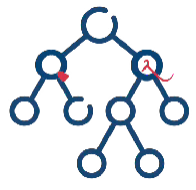
\includegraphics[height=0.9cm]{msca_logo.png}}%
  \end{center}
  \vspace{0.45cm}
  \begin{center}
    \begin{minipage}{0.1\textwidth}\centering
      \href{https://quantlet.com}{
\includegraphics[height=0.9cm]{ql_logo.png}}\end{minipage}%
    \begin{minipage}{0.78\textwidth}\centering
      {\Large\bfseries\usebeamercolor[fg]{title}\inserttitle}\par\vspace{0.25cm}
      {\large\usebeamercolor[fg]{title}\insertsubtitle}\end{minipage}%
    \begin{minipage}{0.1\textwidth}\centering
      \href{https://quantinar.com}{
\includegraphics[height=0.9cm]{qr_logo.png}}\end{minipage}
  \end{center}
  \vfill
  \hspace{0.4cm}{\bfseries\insertauthor}\par\vspace{0.12cm}
  \hspace{0.4cm}\begin{minipage}[t]{0.92\textwidth}\raggedright\footnotesize\insertinstitute\end{minipage}
  \par\vspace{0.4cm}}

% ---------------------------------------------------------------- lecture metadata
\newcommand{\emqashort}{}
\newcommand{\emqanb}{notebooks}
\newcommand{\emqarepo}{https://github.com/danpele/EMQA/tree/main}
% language-dependent labels (English default; \emqaromanian switches to Romanian, call it before \emqalecture)
\newcommand{\txtcourse}{Energy Markets Quantitative Analysis}
\newcommand{\txtlecture}{Lecture}
\newcommand{\txtoutline}{Outline}
\newcommand{\txtintuition}{In one sentence:}
\newcommand{\txtjob}{In practice:}
\newcommand{\txttry}{Experiment yourself:}
\newcommand{\txtwhere}{where}
\newcommand{\txtsim}{SIMULATED DATA (teaching illustration)}
\newcommand{\txtnbsuffix}{}
\newcommand{\txtinstitute}{Bucharest University of Economic Studies, Department of Statistics and Econometrics\\
    Romanian Academy, Institute for Economic Forecasting\\
    IDA Institute Digital Assets \textbullet\ AI4EFin \textbullet\ MSCA Digital Finance}
\newcommand{\emqaromanian}{%
  \renewcommand{\txtcourse}{Analiza cantitativă a piețelor de energie}%
  \renewcommand{\txtlecture}{Cursul}%
  \renewcommand{\txtoutline}{Cuprins}%
  \renewcommand{\txtintuition}{Pe scurt:}%
  \renewcommand{\txtjob}{În practică:}%
  \renewcommand{\txttry}{Exercițiu practic:}%
  \renewcommand{\txtwhere}{unde}%
  \renewcommand{\txtsim}{DATE SIMULATE (doar pentru ilustrare)}%
  \renewcommand{\txtnbsuffix}{\string_ro}%
  \renewcommand{\txtinstitute}{Academia de Studii Economice din București, Departamentul de Statistică și Econometrie\\
    Academia Română, Institutul de Prognoză Economică\\
    IDA Institute Digital Assets \textbullet\ AI4EFin \textbullet\ MSCA Digital Finance}}
\newcommand{\emqalecture}[2]{%
  \renewcommand{\emqashort}{\txtlecture\ #1}%
  \renewcommand{\emqanb}{notebooks/L#1\string_notebook\txtnbsuffix.ipynb}%
  \title[EMQA]{\txtcourse}%
  \subtitle{\txtlecture\ #1: #2}%
  \author{Prof.\ dr.\ Daniel Traian PELE}%
  \institute{\txtinstitute}%
  \date{}}

% ---------------------------------------------------------------- teaching blocks (MBA clarity rule)
% \intuition{one plain sentence}  ->  formula with every symbol defined  ->  real-data example  ->  \manager{one line}
\newcommand{\intuition}[1]{\begin{itemize}\item {\color{MainBlue}\textbf{\txtintuition}}~#1\end{itemize}\vspace{0.6mm}}
\newcommand{\manager}[1]{\colorbox{Forest!10}{\parbox{\dimexpr\linewidth-2\fboxsep\relax}{\footnotesize
  \begin{itemize}\setlength{\itemsep}{0pt}\item \textbf{\color{Forest}\txtjob}~#1\end{itemize}}}}
% Experiment yourself: pointer to the matching notebook section
\newcommand{\tryit}[1]{{\scriptsize\href{\emqarepo/\emqanb}{%
  \raisebox{-0.15em}{
\includegraphics[height=0.85em]{ql_logo.png}}\,\textbf{\txttry}~\color{MainBlue}#1}}}
% bottom row: manager line (left) + experiment pointer (right), pinned to the bottom of the frame
\newcommand{\bottomrow}[2]{\par\vfill\noindent\begin{minipage}[b]{0.72\linewidth}#1\end{minipage}\hfill
  \begin{minipage}[b]{0.26\linewidth}\raggedleft #2\end{minipage}\par\vspace{0.5mm}}
\newcommand{\where}[1]{{\footnotesize\textbf{\txtwhere}~#1\par}}

% ---------------------------------------------------------------- helpers
% chart source line under a figure: \chartsource{Source ...; period ...}
\newcommand{\chartsource}[1]{\par\vspace{1pt}{\scriptsize\color{FooterGray}#1\par}}
% link to code: \quantlet{label}{path inside the repo}
\newcommand{\quantlet}[2]{\par\vspace{1pt}\hfill\href{\emqarepo/#2}{%
  \raisebox{-0.15em}{
\includegraphics[height=0.75em]{ql_logo.png}}\textcolor{MainBlue}{\scriptsize\ #1}}}
\newcommand{\simlabel}{\colorbox{Crimson!12}{\scriptsize\bfseries\color{Crimson}\txtsim}}
\newcommand{\E}{\mathbb{E}}
\newcommand{\Var}{\operatorname{Var}}
\newcommand{\Cov}{\operatorname{Cov}}
\newcommand{\Corr}{\operatorname{Corr}}
\newcommand{\asinh}{\operatorname{asinh}}
\newcommand{\iid}{\overset{\text{i.i.d.}}{\sim}}
\newcommand{\EUR}{EUR}

%   \emqalecture{k}{Lecture title}
% Logos live in lectures/common/logos/, charts in lectures/Lk/charts/.
% Do NOT add \hfuzz / \vfuzz / \hbadness here: overfull boxes must be fixed, not hidden.
% =============================================================================

\usetheme{default}
\setbeamersize{text margin left=7mm, text margin right=7mm}

% ---------------------------------------------------------------- packages
\usepackage[utf8]{inputenc}
\usepackage[T1]{fontenc}
\usepackage{lmodern}
\usepackage{amsmath, amssymb}
\usepackage{mathtools}
\usepackage{bm}
\usepackage{tikz}
\usetikzlibrary{arrows.meta, positioning, calc, shapes.misc}
\usepackage{booktabs}
\usepackage{array}
\usepackage{graphicx}
\usepackage{colortbl}
\usepackage{xcolor}
\usepackage{multicol}
\hypersetup{colorlinks=true, linkcolor=MainBlue, urlcolor=MainBlue, citecolor=MainBlue}
\graphicspath{{../common/logos/}}   % charts are included with their language folder: charts/en/, charts/ro/

% ---------------------------------------------------------------- colours
\definecolor{MainBlue}{RGB}{26, 58, 110}
\definecolor{IDAred}{RGB}{205, 0, 0}
\definecolor{DarkGray}{RGB}{51, 51, 51}
\definecolor{FooterGray}{RGB}{100, 100, 100}
\definecolor{BlockGray}{RGB}{236, 238, 242}
\definecolor{KeynoteGray}{RGB}{218, 218, 218}
\definecolor{Crimson}{RGB}{190, 40, 50}
\definecolor{Forest}{RGB}{30, 110, 50}
\definecolor{Bitter}{RGB}{214, 150, 20}
% chart palette (same hex values as lectures/common/emqa_plot.py)
\definecolor{SerRO}{HTML}{2A78D6}
\definecolor{SerDE}{HTML}{EB6834}
\definecolor{SerHU}{HTML}{1BAF7A}
\definecolor{SerBG}{HTML}{EDA100}

\setbeamertemplate{background}{%
  \begin{tikzpicture}[remember picture, overlay]
    \shade[shading=axis, shading angle=315, top color=white, bottom color=KeynoteGray]
      (current page.south west) rectangle (current page.north east);
  \end{tikzpicture}}
\setbeamercolor{background canvas}{bg=}
\setbeamercolor{structure}{fg=MainBlue}
\setbeamercolor{normal text}{fg=DarkGray}
\setbeamercolor{title}{fg=IDAred}
\setbeamercolor{frametitle}{fg=IDAred, bg=}
\setbeamercolor{block title}{bg=MainBlue, fg=white}
\setbeamercolor{block body}{bg=BlockGray, fg=DarkGray}
\setbeamercolor{block title alerted}{bg=Crimson, fg=white}
\setbeamercolor{block body alerted}{bg=Crimson!7, fg=DarkGray}
\setbeamercolor{block title example}{bg=Forest, fg=white}
\setbeamercolor{block body example}{bg=Forest!7, fg=DarkGray}
\setbeamercolor{item}{fg=MainBlue}
\setbeamerfont{frametitle}{size=\large, series=\bfseries}
\setbeamerfont{block title}{size=\small, series=\bfseries}
\setbeamertemplate{blocks}[rounded][shadow=false]
\setbeamertemplate{itemize item}{\color{MainBlue}$\boxdot$}
\setbeamertemplate{itemize subitem}{\color{MainBlue}\scriptsize$\blacktriangleright$}
% compact two-level lists: level 1 = main point, level 2 = details (no text outside bullets)
\setbeamerfont{itemize/enumerate subbody}{size=\footnotesize}
\setlength{\leftmargini}{1.1em}
\setlength{\leftmarginii}{1.1em}
\setbeamertemplate{itemize/enumerate body begin}{\setlength{\topsep}{0pt}\setlength{\partopsep}{0pt}\setlength{\parskip}{0pt}}
\setbeamertemplate{itemize/enumerate subbody begin}{\setlength{\topsep}{0pt}\setlength{\partopsep}{0pt}\setlength{\itemsep}{0pt}\vspace{-0.4ex}}

\setbeamertemplate{enumerate item}{\color{MainBlue}\insertenumlabel.}
\setlength{\leftmargini}{1.3em}
\setlength{\leftmarginii}{1.2em}
\setbeamertemplate{navigation symbols}{}
\setbeamertemplate{section in toc}{\color{MainBlue}$\blacktriangleright$~\inserttocsection}
\setbeamertemplate{caption}{\raggedright\insertcaption\par}
% frame subtitle = precise citation line under the claim title (Weron style)
\setbeamerfont{framesubtitle}{size=\footnotesize}
\setbeamercolor{framesubtitle}{fg=FooterGray}
% outline that reappears at every section with the current section highlighted
\setbeamertemplate{section in toc shaded}[default][35]
\setbeamertemplate{subsection in toc shaded}[default][35]
\setbeamertemplate{subsection in toc}{\leavevmode\leftskip=2.2em\color{DarkGray}\small\inserttocsubsection\par}
\AtBeginSection[]{{\begin{frame}{\txtoutline}\vspace{2mm}\small
  \tableofcontents[currentsection,hideothersubsections]\end{frame}}}

% ---------------------------------------------------------------- head and foot
\setbeamertemplate{headline}{%
  \vskip10pt%
  \hbox to \paperwidth{\hskip0.5cm%
    {\small\color{FooterGray}\renewcommand{\hyperlink}[2]{##2}\insertsectionhead}%
    \hfill\textcolor{FooterGray}{\small\insertframenumber}\hskip0.5cm}%
  \vskip4pt{\color{FooterGray}\hrule height 0.4pt}}
% footer as in the other courses (MFM, SFM): course name on the left, small sparkline on the right
\setbeamertemplate{footline}{%
  {\color{FooterGray}\hrule height 0.4pt}\vskip4pt%
  \hbox to \paperwidth{\hskip0.5cm%
    \textcolor{FooterGray}{\small\txtcourse}%
    \hfill\raisebox{-0.1em}{\begin{tikzpicture}[x=0.08em, y=0.08em, line width=0.4pt]
      \draw[FooterGray] (0,3) -- (1,4) -- (2,3.5) -- (3,5) -- (4,4) -- (5,6) -- (6,5.5) -- (7,4) -- (8,5) -- (9,7) -- (10,6) -- (11,5) -- (12,6.5) -- (13,8) -- (14,7) -- (15,6) -- (16,7.5) -- (17,9) -- (18,8) -- (19,7) -- (20,8.5) -- (21,10) -- (22,9) -- (23,8) -- (24,9.5);
    \end{tikzpicture}}\hskip0.5cm}%
  \vskip6pt}

% ---------------------------------------------------------------- title page
\defbeamertemplate*{title page}{emqa}[1][]{%
  \vspace{0.15cm}
  \begin{center}
    \href{https://www.ase.ro}{
\includegraphics[height=0.9cm]{ase_logo.png}}\hspace{0.3cm}%
    \href{https://ipe.ro/new}{
\includegraphics[height=0.9cm]{acad_logo.png}}\hspace{0.3cm}%
    \href{https://theida.net}{
\includegraphics[height=0.9cm]{ida_logo.png}}\hspace{0.3cm}%
    \href{https://blockchain-research-center.com}{
\includegraphics[height=0.9cm]{brc_logo.png}}\hspace{0.3cm}%
    \href{https://www.ai4efin.ase.ro}{
\includegraphics[height=0.9cm]{ai4efin_logo.png}}\hspace{0.3cm}%
    \href{https://www.digital-finance-msca.com}{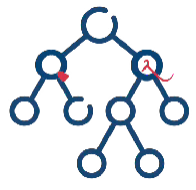
\includegraphics[height=0.9cm]{msca_logo.png}}%
  \end{center}
  \vspace{0.45cm}
  \begin{center}
    \begin{minipage}{0.1\textwidth}\centering
      \href{https://quantlet.com}{
\includegraphics[height=0.9cm]{ql_logo.png}}\end{minipage}%
    \begin{minipage}{0.78\textwidth}\centering
      {\Large\bfseries\usebeamercolor[fg]{title}\inserttitle}\par\vspace{0.25cm}
      {\large\usebeamercolor[fg]{title}\insertsubtitle}\end{minipage}%
    \begin{minipage}{0.1\textwidth}\centering
      \href{https://quantinar.com}{
\includegraphics[height=0.9cm]{qr_logo.png}}\end{minipage}
  \end{center}
  \vfill
  \hspace{0.4cm}{\bfseries\insertauthor}\par\vspace{0.12cm}
  \hspace{0.4cm}\begin{minipage}[t]{0.92\textwidth}\raggedright\footnotesize\insertinstitute\end{minipage}
  \par\vspace{0.4cm}}

% ---------------------------------------------------------------- lecture metadata
\newcommand{\emqashort}{}
\newcommand{\emqanb}{notebooks}
\newcommand{\emqarepo}{https://github.com/danpele/EMQA/tree/main}
% language-dependent labels (English default; \emqaromanian switches to Romanian, call it before \emqalecture)
\newcommand{\txtcourse}{Energy Markets Quantitative Analysis}
\newcommand{\txtlecture}{Lecture}
\newcommand{\txtoutline}{Outline}
\newcommand{\txtintuition}{In one sentence:}
\newcommand{\txtjob}{In practice:}
\newcommand{\txttry}{Experiment yourself:}
\newcommand{\txtwhere}{where}
\newcommand{\txtsim}{SIMULATED DATA (teaching illustration)}
\newcommand{\txtnbsuffix}{}
\newcommand{\txtinstitute}{Bucharest University of Economic Studies, Department of Statistics and Econometrics\\
    Romanian Academy, Institute for Economic Forecasting\\
    IDA Institute Digital Assets \textbullet\ AI4EFin \textbullet\ MSCA Digital Finance}
\newcommand{\emqaromanian}{%
  \renewcommand{\txtcourse}{Analiza cantitativă a piețelor de energie}%
  \renewcommand{\txtlecture}{Cursul}%
  \renewcommand{\txtoutline}{Cuprins}%
  \renewcommand{\txtintuition}{Pe scurt:}%
  \renewcommand{\txtjob}{În practică:}%
  \renewcommand{\txttry}{Exercițiu practic:}%
  \renewcommand{\txtwhere}{unde}%
  \renewcommand{\txtsim}{DATE SIMULATE (doar pentru ilustrare)}%
  \renewcommand{\txtnbsuffix}{\string_ro}%
  \renewcommand{\txtinstitute}{Academia de Studii Economice din București, Departamentul de Statistică și Econometrie\\
    Academia Română, Institutul de Prognoză Economică\\
    IDA Institute Digital Assets \textbullet\ AI4EFin \textbullet\ MSCA Digital Finance}}
\newcommand{\emqalecture}[2]{%
  \renewcommand{\emqashort}{\txtlecture\ #1}%
  \renewcommand{\emqanb}{notebooks/L#1\string_notebook\txtnbsuffix.ipynb}%
  \title[EMQA]{\txtcourse}%
  \subtitle{\txtlecture\ #1: #2}%
  \author{Prof.\ dr.\ Daniel Traian PELE}%
  \institute{\txtinstitute}%
  \date{}}

% ---------------------------------------------------------------- teaching blocks (MBA clarity rule)
% \intuition{one plain sentence}  ->  formula with every symbol defined  ->  real-data example  ->  \manager{one line}
\newcommand{\intuition}[1]{\begin{itemize}\item {\color{MainBlue}\textbf{\txtintuition}}~#1\end{itemize}\vspace{0.6mm}}
\newcommand{\manager}[1]{\colorbox{Forest!10}{\parbox{\dimexpr\linewidth-2\fboxsep\relax}{\footnotesize
  \begin{itemize}\setlength{\itemsep}{0pt}\item \textbf{\color{Forest}\txtjob}~#1\end{itemize}}}}
% Experiment yourself: pointer to the matching notebook section
\newcommand{\tryit}[1]{{\scriptsize\href{\emqarepo/\emqanb}{%
  \raisebox{-0.15em}{
\includegraphics[height=0.85em]{ql_logo.png}}\,\textbf{\txttry}~\color{MainBlue}#1}}}
% bottom row: manager line (left) + experiment pointer (right), pinned to the bottom of the frame
\newcommand{\bottomrow}[2]{\par\vfill\noindent\begin{minipage}[b]{0.72\linewidth}#1\end{minipage}\hfill
  \begin{minipage}[b]{0.26\linewidth}\raggedleft #2\end{minipage}\par\vspace{0.5mm}}
\newcommand{\where}[1]{{\footnotesize\textbf{\txtwhere}~#1\par}}

% ---------------------------------------------------------------- helpers
% chart source line under a figure: \chartsource{Source ...; period ...}
\newcommand{\chartsource}[1]{\par\vspace{1pt}{\scriptsize\color{FooterGray}#1\par}}
% link to code: \quantlet{label}{path inside the repo}
\newcommand{\quantlet}[2]{\par\vspace{1pt}\hfill\href{\emqarepo/#2}{%
  \raisebox{-0.15em}{
\includegraphics[height=0.75em]{ql_logo.png}}\textcolor{MainBlue}{\scriptsize\ #1}}}
\newcommand{\simlabel}{\colorbox{Crimson!12}{\scriptsize\bfseries\color{Crimson}\txtsim}}
\newcommand{\E}{\mathbb{E}}
\newcommand{\Var}{\operatorname{Var}}
\newcommand{\Cov}{\operatorname{Cov}}
\newcommand{\Corr}{\operatorname{Corr}}
\newcommand{\asinh}{\operatorname{asinh}}
\newcommand{\iid}{\overset{\text{i.i.d.}}{\sim}}
\newcommand{\EUR}{EUR}

\usepackage[romanian]{babel}
\emqaromanian
\emqalecture{7}{Învățarea automată pe piețele de energie}
\begin{document}
{\setbeamertemplate{headline}{}\setbeamertemplate{footline}{}
\begin{frame}\titlepage\end{frame}}
% END-FRONT-MATTER

\begin{frame}{Obiectivele cursului}
\small
\begin{itemize}\setlength{\itemsep}{1pt}
  \item Organizarea corectă a unui experiment de învățare automată (ML)
    \begin{itemize}\setlength{\itemsep}{0pt}
      \item Eșantioanele de antrenare, de validare și de test se succed în timp
      \item Prognoza folosește numai informația cunoscută la ora 12:00 a Europei Centrale (CET) în ziua dinaintea livrării
    \end{itemize}
  \item Construirea și calibrarea a două modele pentru cele 24 de prețuri orare ale zilei următoare
    \begin{itemize}\setlength{\itemsep}{0pt}
      \item O rețea neuronală profundă (DNN)
      \item Un ansamblu de arbori de decizie construiți secvențial (gradient boosting)
      \item În plus, un model fundațional preantrenat
    \end{itemize}
  \item Compararea cu modelele de referință din cursul 2, pe același an de test
    \begin{itemize}\setlength{\itemsep}{0pt}
      \item Eroarea absolută medie (MAE), rădăcina erorii pătratice medii (RMSE), MAE relativă (rMAE) și testul Diebold--Mariano (DM)
      \item Combinarea modelelor de învățare automată cu modelele statistice
    \end{itemize}
  \item Explicarea prognozelor, anticiparea vîrfurilor de preț și a prețurilor negative
    \begin{itemize}\setlength{\itemsep}{0pt}
      \item Capcanele care fac un model să pară mai bun decît este
    \end{itemize}
\end{itemize}
\end{frame}

% BEGIN-ABBR

\begin{frame}{Abrevieri (1/2)}
\small
\vspace{-1mm}\begin{columns}[T,onlytextwidth]
\begin{column}{0.49\textwidth}{\scriptsize\renewcommand{\arraystretch}{0.96}\begin{tabular}{@{}>{\bfseries}l@{\ \ }p{0.76\linewidth}@{}}AI & inteligență artificială\\
ARX & model autoregresiv cu variabile exogene\\
AUC & aria de sub curba ROC\\
AW & medierea prognozelor obținute pe mai multe ferestre de calibrare\\
AW-ARX & ARX mediat pe ferestre de calibrare\\
AW-LEAR & LEAR mediat pe ferestre de calibrare\\
CET & ora Europei Centrale\\
CPU & unitatea centrală de procesare (nucleu de procesor)\\
DM & testul Diebold--Mariano\\
DNN & rețea neuronală profundă\\\end{tabular}}\end{column}
\begin{column}{0.49\textwidth}{\scriptsize\renewcommand{\arraystretch}{0.96}\begin{tabular}{@{}>{\bfseries}l@{\ \ }p{0.76\linewidth}@{}}DST & ora de vară\\
ENTSO-E & Rețeaua europeană a operatorilor de transport și de sistem pentru energie electrică\\
ETC & titlu tranzacționat la bursă, garantat cu mărfuri (exchange-traded commodity)\\
EUA & certificat de emisii al UE (1 t CO$_2$)\\
EUR & euro\\
GBM & gradient boosting (ansamblu de arbori de decizie construiți secvențial)\\
GW & gigawatt\\
ISE & Institutul Fraunhofer pentru Sisteme de Energie Solară\\
LASSO & operatorul de contracție și selecție în normă absolută\\\end{tabular}}\end{column}
\end{columns}
\end{frame}

\begin{frame}{Abrevieri (2/2)}
\small
\vspace{-1mm}\begin{columns}[T,onlytextwidth]
\begin{column}{0.49\textwidth}{\scriptsize\renewcommand{\arraystretch}{0.96}\begin{tabular}{@{}>{\bfseries}l@{\ \ }p{0.76\linewidth}@{}}LEAR & autoregresie estimată cu LASSO\\
MAD & abaterea absolută mediană\\
MAE & eroarea absolută medie\\
ML & învățare automată\\
MLP & perceptron multistrat (rețea neuronală directă)\\
MW & megawatt\\
MWh & megawatt-oră\\
OPCOM & operatorul pieței de energie electrică și de gaze naturale din România\\
PZU & piața pentru ziua următoare\\
ReLU & unitate liniară rectificată (rectified linear unit)\\\end{tabular}}\end{column}
\begin{column}{0.49\textwidth}{\scriptsize\renewcommand{\arraystretch}{0.96}\begin{tabular}{@{}>{\bfseries}l@{\ \ }p{0.76\linewidth}@{}}RES & surse regenerabile de energie (aici: eolian + solar)\\
rMAE & MAE relativă (MAE a modelului / MAE a modelului naiv)\\
RMSE & rădăcina erorii pătratice medii\\
RO & România (zonă de ofertare)\\
ROC & caracteristica de operare a receptorului (receiver operating characteristic)\\
SHAP & explicații aditive bazate pe valorile Shapley (SHapley Additive exPlanations)\\
TSO & operator de transport și de sistem\\
UE & Uniunea Europeană\\
XGBoost & eXtreme Gradient Boosting (bibliotecă de programe)\\\end{tabular}}\end{column}
\end{columns}
\end{frame}

% END-ABBR

\begin{frame}{Aceleași date și același an de test ca în cursul 2, plus un an de validare}
\footnotesize
{\scriptsize\renewcommand{\arraystretch}{1.0}\setlength{\tabcolsep}{4pt}
\begin{tabular}{@{}p{0.24\textwidth}p{0.70\textwidth}@{}}\toprule
Element & Alegerea din acest curs \\ \midrule
Variabila prognozată & prețul orar de pe piața pentru ziua următoare (PZU) din România (RO), administrată de operatorul pieței de energie electrică și de gaze naturale (OPCOM) \\
Variabile explicative (ca în cursul 2) & prețurile pînă în ziua $d-1$; consumul, producția eoliană și solară, hidro, nucleară și importul net pînă în ziua $d-2$, de la Rețeaua europeană a operatorilor de transport și de sistem pentru energie electrică (ENTSO-E); prețul certificatelor de emisii (EUA) ale Uniunii Europene (UE), printr-un titlu tranzacționat la bursă (ETC) \\
Antrenare & de la 8 ianuarie 2022; crește cu o lună la fiecare reestimare \\
Anul de validare & 1 noiembrie 2024 -- 31 octombrie 2025: folosit numai pentru alegerea setărilor modelelor \\
Anul de test & 1 noiembrie 2025 -- 31 octombrie 2026, 8\,760 de ore, modele reestimate lunar \\
\bottomrule\end{tabular}}
\vspace{1mm}
\begin{itemize}\setlength{\itemsep}{1pt}
  \item \textbf{Date pînă la 31 octombrie 2026}
    \begin{itemize}\setlength{\itemsep}{0pt}
      \item Descărcate la 4 noiembrie 2026 de pe energy-charts.info (Fraunhofer ISE) și Yahoo Finance
    \end{itemize}
  \item \textbf{Modelele de referință}: prognozele din cursul 2, preluate din fișierele acestuia
    \begin{itemize}\setlength{\itemsep}{0pt}
      \item Modelul naiv; modelul autoregresiv cu variabile exogene (ARX); operatorul de contracție și selecție în normă absolută (LASSO)
      \item Autoregresia estimată cu LASSO (LEAR); ARX mediat pe mai multe ferestre de calibrare (AW-ARX), LEAR la fel (AW-LEAR); ansamblul de 4 modele
    \end{itemize}
\end{itemize}
\par\vfill\noindent{\scriptsize\color{FooterGray}}\hfill\tryit{notebook-ul Jupyter, secțiunea 1}\par\vspace{0.5mm}
\end{frame}


\section{Învățarea automată, evaluată corect}

\begin{frame}{Învățarea automată cîștigă flexibilitate, dar plătește prin varianță}
\footnotesize
\intuition{Un model flexibil poate învăța praguri și interacțiuni pe care LEAR nu le vede, dar poate învăța și zgomotul din anii de antrenare.}
\begin{columns}[T,onlytextwidth]
\begin{column}{0.52\textwidth}
\[ \hat\theta=\arg\min_{\theta}\ \underbrace{\frac1n\sum_{i=1}^{n}\ell\big(Y_i,f_\theta(\mathbf x_i)\big)}_{\text{potrivirea pe zilele de antrenare}}+\underbrace{\lambda\,\Omega(\theta)}_{\text{penalizare}} \]{\footnotesize\begin{itemize}\setlength{\itemsep}{0pt}
  \item \textbf{\txtwhere}
    \begin{itemize}\setlength{\itemsep}{0pt}
      \item $f_\theta$ = modelul, cu parametrii $\theta$
      \item $\mathbf x_i$ = variabilele cunoscute la închiderea licitației
      \item $Y_i$ = prețul
      \item $\ell$ = funcția de pierdere, aici eroarea absolută
      \item $\Omega$ = complexitatea modelului, iar $\lambda$ = ponderea ei.
    \end{itemize}
\end{itemize}\par}
\end{column}
\begin{column}{0.45\textwidth}
\begin{itemize}\setlength{\itemsep}{1pt}
  \item \textbf{Cît de flexibile sînt modelele noastre?}
    \begin{itemize}\setlength{\itemsep}{0pt}
      \item LEAR: cel mult 247 de coeficienți pentru fiecare oră
      \item Rețeaua DNN: 141\,336 de parametri, pentru 1\,727 de zile de antrenare la ultima reestimare
    \end{itemize}
  \item \textbf{Consecința}
    \begin{itemize}\setlength{\itemsep}{0pt}
      \item Eroarea pe datele de antrenare nu spune nimic despre viitor; modelul poate fi judecat numai pe date pe care nu le-a văzut
    \end{itemize}
\end{itemize}
\end{column}
\end{columns}
\par\vfill\manager{întrebați furnizorul de prognoze cîți parametri are modelul pentru fiecare zi de istoric și pe ce zile a fost măsurată eroarea.}\par\vspace{0.5mm}
\par\vfill\noindent{\scriptsize\color{FooterGray}(Hastie, Tibshirani \& Friedman, 2009; Lago et al., 2021, APEN)}\hfill\tryit{notebook-ul Jupyter, secțiunea 1}\par\vspace{0.5mm}
\end{frame}

\begin{frame}{Trei eșantioane în ordine cronologică: antrenare, validare, test}
\small
\begin{center}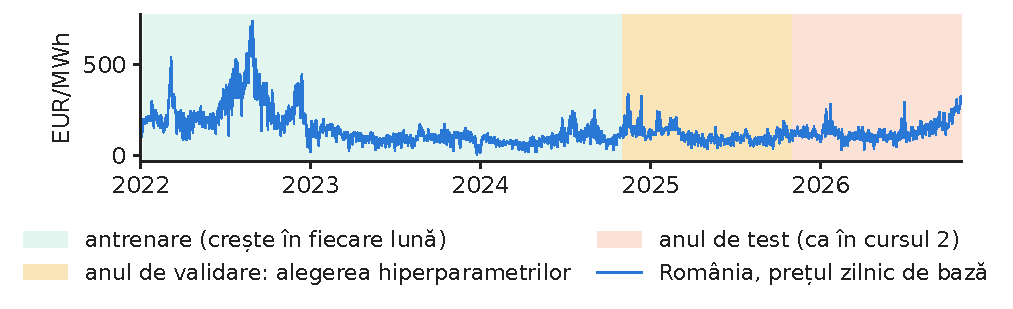
\includegraphics[width=\textwidth,height=0.383\textheight,keepaspectratio]{charts/ro/split_ml.pdf}\end{center}\vspace{-3mm}
\chartsource{Sursa: energy-charts.info (Fraunhofer ISE): prețurile PZU ale OPCOM pentru România. Date: preț zilnic de bază, 2022-01-01 - 2026-10-31, zile de livrare CET.}
\vspace{0.5mm}
\begin{itemize}\setlength{\itemsep}{0pt}
  \item \textbf{Anul de validare}: se compară 25 de setări pentru fiecare model, reestimate la fiecare 3 luni
    \begin{itemize}\setlength{\itemsep}{0pt}
      \item Setarea cu cea mai mică MAE este fixată înainte de începutul anului de test
    \end{itemize}
  \item \textbf{Anul de test}: modelele sînt reestimate la începutul fiecărei luni, pe toate zilele anterioare
    \begin{itemize}\setlength{\itemsep}{0pt}
      \item Nu se folosește pentru nicio alegere; este același an ca în cursul 2, deci erorile se pot compara direct
    \end{itemize}
\end{itemize}
\par\vfill\manager{tratați anul de test ca pe un plic sigilat: se deschide o singură dată, după ce toate alegerile au fost făcute.}\par\vspace{0.5mm}
\par\vfill\noindent{\scriptsize\color{FooterGray}(Bergmeir \& Benítez, 2012, Inf.\ Sci.; Lago et al., 2021, APEN)}\hfill\tryit{notebook-ul Jupyter, secțiunea 1}\par\vspace{0.5mm}
\end{frame}

\begin{frame}{Hiperparametrii se aleg prin căutare aleatoare pe anul de validare}
\footnotesize
\intuition{Setări precum numărul de neuroni sau de arbori nu sînt estimate de model; încercăm mai multe și o păstrăm pe cea care prognozează cel mai bine zilele nevăzute.}
\begin{columns}[T,onlytextwidth]
\begin{column}{0.55\textwidth}
\[ \gamma^{*}=\arg\min_{\gamma\in\{\gamma_0,\dots,\gamma_{24}\}}\ \frac{1}{24\,|\mathcal V|}\sum_{d\in\mathcal V}\sum_{h=0}^{23}\big|P_{d,h}-\hat P_{d,h}(\gamma)\big| \]{\footnotesize\begin{itemize}\setlength{\itemsep}{0pt}
  \item \textbf{\txtwhere}
    \begin{itemize}\setlength{\itemsep}{0pt}
      \item $\gamma$ = o setare (vectorul hiperparametrilor)
      \item $\gamma_0$ = setarea din cursul 2, celelalte extrase aleator
      \item $\mathcal V$ = zilele anului de validare
      \item $\hat P_{d,h}(\gamma)$ = prognoza cu setarea $\gamma$.
    \end{itemize}
\end{itemize}\par}
\end{column}
\begin{column}{0.42\textwidth}
\begin{itemize}\setlength{\itemsep}{1pt}
  \item \textbf{De ce aleator și nu pe o grilă completă}
    \begin{itemize}\setlength{\itemsep}{0pt}
      \item Doar cîteva setări contează cu adevărat; extragerile aleatoare le acoperă mai bine, cu același număr de încercări
    \end{itemize}
  \item \textbf{Bugetul nostru}
    \begin{itemize}\setlength{\itemsep}{0pt}
      \item 24 de setări aleatoare și setarea din cursul 2, pentru fiecare dintre cele două modele
      \item 7{,}3 minute pe un nucleu al unității centrale de procesare (CPU)
    \end{itemize}
\end{itemize}
\end{column}
\end{columns}
\par\vfill\manager{o căutare modestă, dar documentată, este suficientă
    \begin{itemize}\setlength{\itemsep}{0pt}
      \item O căutare fără un eșantion de validare separat nu este o căutare, ci o scurgere de informație.
    \end{itemize}}\par\vspace{0.5mm}
\par\vfill\noindent{\scriptsize\color{FooterGray}(Bergstra \& Bengio, 2012, JMLR)}\hfill\tryit{notebook-ul Jupyter, secțiunea 2}\par\vspace{0.5mm}
\end{frame}


\section{Rețele neuronale profunde}

\begin{frame}{O rețea neuronală înlănțuie regresii, fiecare urmată de o funcție neliniară}
\footnotesize
\intuition{Fiecare neuron transformă neliniar o combinație liniară a intrărilor; stratul de ieșire dă deodată cele 24 de prețuri ale zilei $d$.}
\begin{columns}[T,onlytextwidth]
\begin{column}{0.56\textwidth}
\[ \mathbf z=\phi\big(W_1\mathbf x_d+\mathbf b_1\big),\qquad \hat{\mathbf Y}_d=W_2\,\mathbf z+\mathbf b_2\in\mathbb R^{24} \]\[ \phi(u)=\max(0,u)\quad\text{sau}\quad \phi(u)=\ln(1+e^{u}) \]{\footnotesize\begin{itemize}\setlength{\itemsep}{0pt}
  \item \textbf{\txtwhere}
    \begin{itemize}\setlength{\itemsep}{0pt}
      \item $\mathbf x_d$ = intrările zilei $d$ (prețuri, consum, eolian și solar, variabile fundamentale, ziua săptămînii)
      \item $W_1,W_2$ = ponderi, $\mathbf b_1,\mathbf b_2$ = termeni liberi
      \item $\phi$ = unitatea liniară rectificată (ReLU) sau varianta netedă (softplus)
      \item $\hat{\mathbf Y}_d$ = prețurile transformate cu asinh (cursul 2).
    \end{itemize}
\end{itemize}\par}
\end{column}
\begin{column}{0.41\textwidth}
\begin{itemize}\setlength{\itemsep}{1pt}
  \item \textbf{Rețeaua noastră} (aleasă pe anul de validare)
    \begin{itemize}\setlength{\itemsep}{0pt}
      \item 251 de intrări, un strat ascuns de 512 de neuroni, funcția softplus, 24 de ieșiri
      \item 141\,336 de parametri; rețelele cu două straturi au fost mai slabe la validare
    \end{itemize}
  \item \textbf{Mai bună decît în cursul 2}
    \begin{itemize}\setlength{\itemsep}{0pt}
      \item Perceptronul multistrat (MLP): MAE 25{,}54; rețeaua de acum: 22{,}95 EUR/MWh
    \end{itemize}
\end{itemize}
\end{column}
\end{columns}
\par\vfill\manager{o rețea neuronală este o regresie cu mult mai mulți coeficienți: are nevoie de aceeași disciplină a datelor, nu de mai puțină.}\par\vspace{0.5mm}
\par\vfill\noindent{\scriptsize\color{FooterGray}(Lago, Marcjasz, De Schutter \& Weron, 2021, APEN)}\hfill\tryit{notebook-ul Jupyter, secțiunea 2}\par\vspace{0.5mm}
\end{frame}

\begin{frame}{Antrenarea: pași mici împotriva erorii, opriți la timp}
\footnotesize
\intuition{Ponderile se modifică puțin, în direcția care reduce eroarea pe un grup aleator de zile; ne oprim cînd eroarea pe zilele mai recente nu mai scade.}
\begin{columns}[T,onlytextwidth]
\begin{column}{0.52\textwidth}
\[ \mathcal L(\theta)=\frac{1}{24\,|B|}\sum_{d\in B}\sum_{h=0}^{23}\big|Y_{d,h}-\hat Y_{d,h}(\theta)\big| \]\[ \theta\leftarrow\theta-\eta\,\widehat{\nabla\mathcal L} \]{\footnotesize\begin{itemize}\setlength{\itemsep}{0pt}
  \item \textbf{\txtwhere}
    \begin{itemize}\setlength{\itemsep}{0pt}
      \item $B$ = un grup de 64 de zile (mini-batch)
      \item $\eta$ = rata de învățare ($3\cdot10^{-4}$)
      \item $\widehat{\nabla\mathcal L}$ = gradientul, rescalat prin metoda Adam
      \item O epocă = o parcurgere a tuturor zilelor de antrenare.
    \end{itemize}
\end{itemize}\par}
\end{column}
\begin{column}{0.45\textwidth}
\begin{itemize}\setlength{\itemsep}{1pt}
  \item \textbf{Oprirea timpurie (early stopping)}
    \begin{itemize}\setlength{\itemsep}{0pt}
      \item Antrenare pe primele 85\% din zile, urmărirea erorii pe ultimele 15\%
      \item Se păstrează epoca cea mai bună, apoi rețeaua se reestimează pe toate zilele, cu același număr de epoci
    \end{itemize}
  \item \textbf{Pe datele noastre}
    \begin{itemize}\setlength{\itemsep}{0pt}
      \item Epocile păstrate: mediana 56, între 23 și 92 (12 reestimări $\times$ 4 inițializări)
      \item Dropout: în timpul antrenării, fiecare neuron este dezactivat aleator, cu probabilitatea 0{,}1
    \end{itemize}
\end{itemize}
\end{column}
\end{columns}
\par\vfill\manager{regula de oprire folosește numai zile din trecut: face parte din model și se verifică la fel ca restul.}\par\vspace{0.5mm}
\par\vfill\noindent{\scriptsize\color{FooterGray}(Kingma \& Ba, 2015, ICLR; Srivastava et al., 2014, JMLR)}\hfill\tryit{notebook-ul Jupyter, secțiunea 2}\par\vspace{0.5mm}
\end{frame}

\begin{frame}{Oprirea timpurie: ne oprim cînd eroarea pe zilele recente nu mai scade}
\small
\begin{center}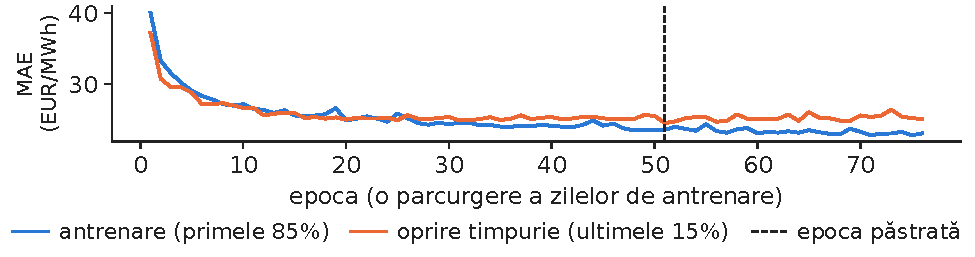
\includegraphics[width=\textwidth,height=0.350\textheight,keepaspectratio]{charts/ro/learning_curve.pdf}\end{center}\vspace{-3mm}
\chartsource{Sursa: energy-charts.info (Fraunhofer ISE): prețuri OPCOM; consum, producție și fluxuri ENTSO-E; Yahoo Finance (EUA ETC). Date: rețeaua DNN aleasă, reestimarea pentru 2026-10, inițializarea 1.}
\vspace{0.5mm}
\begin{itemize}\setlength{\itemsep}{0pt}
  \item Reestimarea pentru octombrie 2026: eroarea pe ultimele 15\% din zile este minimă la epoca 51 (24{,}50 EUR/MWh)
    \begin{itemize}\setlength{\itemsep}{0pt}
      \item Antrenarea se oprește la epoca 76
    \end{itemize}
  \item După acest punct, rețeaua reproduce tot mai bine trecutul și tot mai slab zilele recente
    \begin{itemize}\setlength{\itemsep}{0pt}
      \item Începe să memoreze
    \end{itemize}
\end{itemize}
\par\vfill\manager{dacă un furnizor nu vă poate arăta această curbă, rețeaua a fost probabil antrenată pînă a reprodus trecutul.}\par\vspace{0.5mm}
\par\vfill\noindent{\scriptsize\color{FooterGray}(calcule proprii; rețeaua DNN aleasă, inițializarea 1)}\hfill\tryit{notebook-ul Jupyter, secțiunea 2}\par\vspace{0.5mm}
\end{frame}

\begin{frame}{Căutarea aleatoare reduce eroarea de validare a ambelor modele}
\small
\begin{center}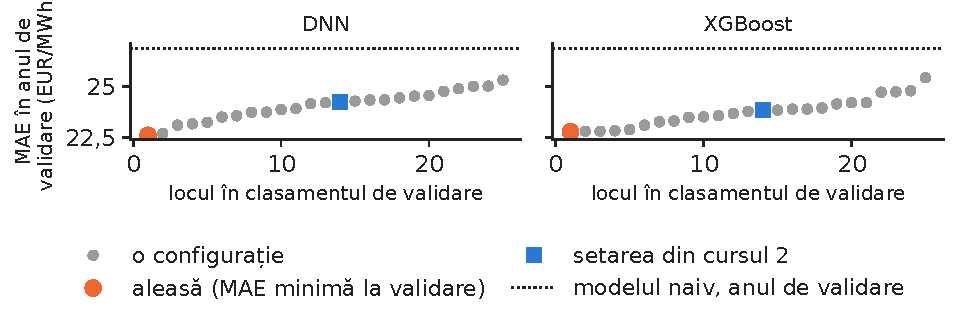
\includegraphics[width=\textwidth,height=0.369\textheight,keepaspectratio]{charts/ro/search.pdf}\end{center}\vspace{-3mm}
\chartsource{Sursa: energy-charts.info (Fraunhofer ISE): prețuri OPCOM; consum, producție și fluxuri ENTSO-E; Yahoo Finance (EUA ETC). Date: anul de validare 2024-11-01 - 2025-10-31; 25 de configurații pe model, reestimare trimestrială.}
\vspace{0.5mm}
\begin{itemize}\setlength{\itemsep}{0pt}
  \item \textbf{DNN}: cea mai bună setare are MAE 22{,}59 EUR/MWh; setarea din cursul 2, 24{,}24, locul 14 din 25
    \begin{itemize}\setlength{\itemsep}{0pt}
      \item \textbf{eXtreme Gradient Boosting (XGBoost)}: 22{,}76 față de 23{,}83 (locul 14)
    \end{itemize}
  \item Toate cele 25 de setări ale ambelor modele sînt mai precise decît modelul naiv în anul de validare (26{,}90 EUR/MWh)
\end{itemize}
\par\vfill\manager{prevedeți un an de validare pentru calibrare înainte de a avea încredere într-o prognoză de învățare automată.}\par\vspace{0.5mm}
\par\vfill\noindent{\scriptsize\color{FooterGray}(calcule proprii; anul de validare 1 noiembrie 2024 -- 31 octombrie 2025)}\hfill\tryit{notebook-ul Jupyter, secțiunea 2}\par\vspace{0.5mm}
\end{frame}


\section{Gradient boosting și modele fundaționale}

\begin{frame}{Un arbore de regresie împarte intrările în căsuțe, cu cîte un preț fiecare}
\footnotesize
\intuition{Un arbore pune întrebări cu răspuns da/nu; fiecare frunză finală conține o valoare, deci pragurile și interacțiunile apar de la sine.}
\begin{columns}[T,onlytextwidth]
\begin{column}{0.60\textwidth}
\[ f(\mathbf x)=\textstyle\sum_{j=1}^{J}w_j\,\mathbb 1\{\mathbf x\in R_j\} \]\vspace{-1mm}\[ \text{Gain}=\frac{G_L^2}{H_L+\lambda}+\frac{G_R^2}{H_R+\lambda}-\frac{(G_L+G_R)^2}{H_L+H_R+\lambda}-\gamma \]{\footnotesize\begin{itemize}\setlength{\itemsep}{0pt}
  \item \textbf{\txtwhere}
    \begin{itemize}\setlength{\itemsep}{0pt}
      \item $R_j$ = frunza $j$, $w_j$ = valoarea ei
      \item $G$, $H$ = sumele derivatelor de ordinul 1 și 2 ale pierderii, la stînga ($L$) și la dreapta ($R$)
      \item $\lambda$, $\gamma$ = penalizări
      \item Se alege împărțirea cu cel mai mare cîștig.
    \end{itemize}
\end{itemize}\par}
\end{column}
\begin{column}{0.37\textwidth}
\begin{itemize}\setlength{\itemsep}{1pt}
  \item \textbf{Pe datele noastre} (reestimarea pentru octombrie 2026)
    \begin{itemize}\setlength{\itemsep}{0pt}
      \item Primul arbore întreabă: prețul din $d-1$, aceeași oră, este sub 119{,}5 EUR/MWh?
      \item 233 de frunze; modelul adună 1\,500 de arbori
    \end{itemize}
\end{itemize}
\end{column}
\end{columns}
\par\vfill\manager{un arbore gîndește ca un trader: dacă ieri prețul a trecut de un prag, diseară urmează o primă.}\par\vspace{0.5mm}
\par\vfill\noindent{\scriptsize\color{FooterGray}(Chen \& Guestrin, 2016, KDD; Hastie et al., 2009)}\hfill\tryit{notebook-ul Jupyter, secțiunea 3}\par\vspace{0.5mm}
\end{frame}

\begin{frame}{Gradient boosting: fiecare arbore nou corectează erorile rămase}
\footnotesize
\intuition{Potrivim un arbore mic pe ceea ce este încă greșit, îl adăugăm cu o pondere mică și repetăm de o mie de ori.}
\begin{columns}[T,onlytextwidth]
\begin{column}{0.57\textwidth}
\[ F_m(\mathbf x)=F_{m-1}(\mathbf x)+\eta\,f_m(\mathbf x),\qquad w_j^{*}=-\frac{G_j}{H_j+\lambda} \]\[ \min\ \textstyle\sum_{i}\ell\big(Y_i,F_M(\mathbf x_i)\big)+\sum_{m}\big(\gamma J_m+\tfrac{\lambda}{2}\sum_j w_{mj}^2\big) \]{\footnotesize\begin{itemize}\setlength{\itemsep}{0pt}
  \item \textbf{\txtwhere}
    \begin{itemize}\setlength{\itemsep}{0pt}
      \item $F_m$ = prognoza după $m$ arbori
      \item $f_m$ = arborele $m$, cu $J_m$ frunze
      \item $\eta$ = rata de învățare
      \item $w_j^{*}$ = valoarea optimă a frunzei $j$ (anexa B)
      \item $\ell$ = eroarea absolută.
    \end{itemize}
\end{itemize}\par}
\end{column}
\begin{column}{0.40\textwidth}
\begin{itemize}\setlength{\itemsep}{1pt}
  \item \textbf{Setarea aleasă pe anul de validare}
    \begin{itemize}\setlength{\itemsep}{0pt}
      \item 1\,500 de arbori de adîncime 8, $\eta$ = 0{,}02, fiecare pe o fracțiune 0{,}8 din rînduri
    \end{itemize}
  \item \textbf{Anul de test}
    \begin{itemize}\setlength{\itemsep}{0pt}
      \item MAE 23{,}26 EUR/MWh; modelul gradient boosting (GBM) necalibrat din cursul 2: 24{,}05 (DM: $p<0{,}001$)
      \item AW-LEAR (22{,}53) rămîne mai precis (DM: $p$ = 0{,}016)
    \end{itemize}
\end{itemize}
\end{column}
\end{columns}
\par\vfill\manager{calibrarea contează mai mult decît programul: același tip de arbori a cîștigat aproape un euro pe MWh prin setări bune.}\par\vspace{0.5mm}
\par\vfill\noindent{\scriptsize\color{FooterGray}(Friedman, 2001, Ann.\ Stat.; Chen \& Guestrin, 2016, KDD)}\hfill\tryit{notebook-ul Jupyter, secțiunea 3}\par\vspace{0.5mm}
\end{frame}

\begin{frame}{Modelele fundaționale prognozează prețurile fără nicio antrenare}
\footnotesize
\intuition{Modelele Chronos au fost antrenate de Amazon pe colecții mari de serii de timp; noi le dăm doar prețurile recente și le cerem următoarele 24 de ore (fără reantrenare, zero-shot).}
\begin{columns}[T,onlytextwidth]
\begin{column}{0.52\textwidth}
\[ \big(\hat q^{\tau}_{d,h}\big)_{h=0,\dots,23}^{\tau=0{,}1;\,0{,}5;\,0{,}9}=g\big(P_{t-2047},\dots,P_{t}\big) \]{\footnotesize\begin{itemize}\setlength{\itemsep}{0pt}
  \item \textbf{\txtwhere}
    \begin{itemize}\setlength{\itemsep}{0pt}
      \item $P_{t-2047},\dots,P_t$ = ultimele 2048 de prețuri orare, pînă la sfîrșitul zilei $d-1$ (85 de zile)
      \item $g$ = rețeaua preantrenată, folosită ca atare
      \item $\hat q^{\tau}$ = cuantilele prognozate
      \item Prognoza punctuală este mediana $\hat q^{0{,}5}$.
    \end{itemize}
\end{itemize}\par}
\end{column}
\begin{column}{0.45\textwidth}
\begin{itemize}\setlength{\itemsep}{1pt}
  \item \textbf{Anul de test}, numai cu prețuri, fără variabile fundamentale
    \begin{itemize}\setlength{\itemsep}{0pt}
      \item Chronos-2: MAE 20{,}82; Chronos-Bolt: 22{,}15; AW-LEAR: 22{,}53 EUR/MWh
      \item Chronos-2 este mai precis decît AW-LEAR: DM, $p<0{,}001$; în toate cele 24 de ore
    \end{itemize}
  \item \textbf{Robustețe}
    \begin{itemize}\setlength{\itemsep}{0pt}
      \item În anul de validare: Chronos-2 21{,}05, cea mai bună rețea DNN calibrată 22{,}59
      \item Publicat în octombrie 2025, înaintea anului de test
    \end{itemize}
\end{itemize}
\end{column}
\end{columns}
\par\vfill\manager{testați un model fundațional înainte de a construi propria rețea: costă puțin, iar aici a fost cel mai precis model individual.}\par\vspace{0.5mm}
\par\vfill\noindent{\scriptsize\color{FooterGray}(Ansari et al., 2024, TMLR; Ansari et al., 2025, arXiv)}\hfill\tryit{notebook-ul Jupyter, secțiunea 4}\par\vspace{0.5mm}
\end{frame}

\begin{frame}{Chronos-2 este mai precis decît AW-LEAR în fiecare oră a zilei}
\small
\begin{center}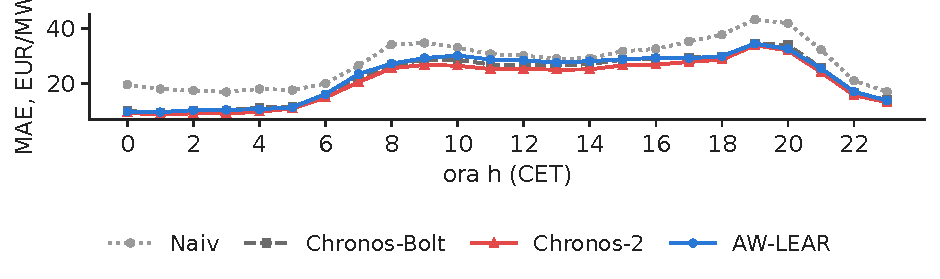
\includegraphics[width=\textwidth,height=0.427\textheight,keepaspectratio]{charts/ro/foundation_hour.pdf}\end{center}\vspace{-3mm}
\chartsource{Sursa: energy-charts.info (Fraunhofer ISE): prețurile PZU ale OPCOM pentru România. Date: anul de test 2025-11-01 - 2026-10-31; fără reantrenare, context = ultimele 2048 de prețuri orare.}
\vspace{0.5mm}
\begin{itemize}\setlength{\itemsep}{0pt}
  \item Chronos-Bolt, mai mic și mai vechi, este la egalitate cu AW-LEAR (DM: $p$ = 0{,}220)
  \item Intervalul 10\%--90\% al modelului Chronos-2 conține 76{,}5\% din prețuri, nu 80\%: este prea îngust
\end{itemize}
\par\vfill\manager{folosiți mediana
    \begin{itemize}\setlength{\itemsep}{0pt}
      \item Recalibrați intervalele (cursul 2) înainte de a dimensiona riscul cu ele.
    \end{itemize}}\par\vspace{0.5mm}
\par\vfill\noindent{\scriptsize\color{FooterGray}(calcule proprii, anul de test 1 noiembrie 2025 -- 31 octombrie 2026)}\hfill\tryit{notebook-ul Jupyter, secțiunea 4}\par\vspace{0.5mm}
\end{frame}


\section{Comparație corectă, combinare și cost}

\begin{frame}{Clasamentul: Chronos-2 este cel mai bun model individual}
\small
\begin{center}{\scriptsize\renewcommand{\arraystretch}{0.96}\setlength{\tabcolsep}{4pt}
\begin{tabular}{@{}lrrrrr@{}}\toprule
Model & MAE & RMSE & rMAE & față de AW-LEAR, \% & DM, $p$ \\ \midrule
Naiv & \cellcolor{Crimson!55}27{,}82 & \cellcolor{Crimson!55}44{,}54 & \cellcolor{Crimson!55}1{,}000 & \cellcolor{Crimson!55}\ensuremath{-}23{,}5 & -- \\
AW-ARX & \cellcolor{Forest!32}22{,}30 & \cellcolor{Forest!31}36{,}34 & \cellcolor{Forest!31}0{,}802 & \cellcolor{Forest!32}\ensuremath{+}1{,}0 & 0{,}203 \\
AW-LEAR & \cellcolor{Forest!28}22{,}53 & \cellcolor{Forest!31}36{,}35 & \cellcolor{Forest!28}0{,}810 & \cellcolor{Forest!28}\ensuremath{+}0{,}0 & -- \\
Ansamblul de 4 (cursul 2) & \cellcolor{Forest!34}22{,}13 & \cellcolor{Forest!38}35{,}76 & \cellcolor{Forest!34}0{,}795 & \cellcolor{Forest!34}\ensuremath{+}1{,}8 & 0{,}014 \\
GBM (cursul 2) & \cellcolor{Forest!4}24{,}05 & \cellcolor{Forest!17}37{,}73 & \cellcolor{Forest!4}0{,}864 & \cellcolor{Forest!4}\ensuremath{-}6{,}7 & 1{,}000 \\
MLP (cursul 2) & \cellcolor{Crimson!19}25{,}54 & \cellcolor{Crimson!8}40{,}05 & \cellcolor{Crimson!19}0{,}918 & \cellcolor{Crimson!19}\ensuremath{-}13{,}3 & 1{,}000 \\
XGBoost, calibrat & \cellcolor{Forest!17}23{,}26 & \cellcolor{Forest!25}36{,}94 & \cellcolor{Forest!17}0{,}836 & \cellcolor{Forest!17}\ensuremath{-}3{,}2 & 0{,}984 \\
DNN, calibrată & \cellcolor{Forest!21}22{,}95 & \cellcolor{Forest!31}36{,}42 & \cellcolor{Forest!21}0{,}825 & \cellcolor{Forest!22}\ensuremath{-}1{,}8 & 0{,}944 \\
Chronos-Bolt, fără antrenare & \cellcolor{Forest!34}22{,}15 & \cellcolor{Forest!39}35{,}65 & \cellcolor{Forest!34}0{,}796 & \cellcolor{Forest!34}\ensuremath{+}1{,}7 & 0{,}220 \\
Chronos-2, fără antrenare & \cellcolor{Forest!55}20{,}82 & \cellcolor{Forest!53}34{,}32 & \cellcolor{Forest!55}0{,}748 & \cellcolor{Forest!55}\ensuremath{+}7{,}6 & $<$0{,}001 \\
AW-LEAR + DNN + XGBoost & \cellcolor{Forest!37}21{,}97 & \cellcolor{Forest!41}35{,}42 & \cellcolor{Forest!37}0{,}790 & \cellcolor{Forest!37}\ensuremath{+}2{,}5 & 0{,}001 \\
AW-ARX + AW-LEAR + DNN + XGBoost & \cellcolor{Forest!41}21{,}69 & \cellcolor{Forest!43}35{,}25 & \cellcolor{Forest!41}0{,}779 & \cellcolor{Forest!42}\ensuremath{+}3{,}8 & $<$0{,}001 \\
AW-LEAR + Chronos-2 & \cellcolor{Forest!55}20{,}81 & \cellcolor{Forest!55}34{,}11 & \cellcolor{Forest!55}0{,}748 & \cellcolor{Forest!55}\ensuremath{+}7{,}6 & -- \\
Ansamblul de 5 (cu Chronos-2) & \cellcolor{Forest!50}21{,}12 & \cellcolor{Forest!51}34{,}50 & \cellcolor{Forest!50}0{,}759 & \cellcolor{Forest!50}\ensuremath{+}6{,}3 & $<$0{,}001 \\
\bottomrule\end{tabular}}\end{center}\vspace{-2mm}
\par\vspace{0.5mm}{\scriptsize \begin{itemize}\setlength{\itemsep}{0pt}
  \item Rădăcina erorii pătratice medii (RMSE); MAE relativă (rMAE) = MAE / MAE a modelului naiv; verde = mai precis, pe fiecare coloană.
  \item DM, $p$: test unilateral că modelul este mai precis decît AW-LEAR (eroarea absolută medie zilnică, varianță Newey--West, ca în cursul 2).
\end{itemize}}
\par\vfill\noindent{\scriptsize\color{FooterGray}(calcule proprii, anul de test 1 noiembrie 2025 -- 31 octombrie 2026)}\hfill\tryit{notebook-ul Jupyter, secțiunea 5}\par\vspace{0.5mm}
\end{frame}

\begin{frame}{Testele DM: combinațiile cu ML depășesc semnificativ AW-LEAR}
\small
\begin{center}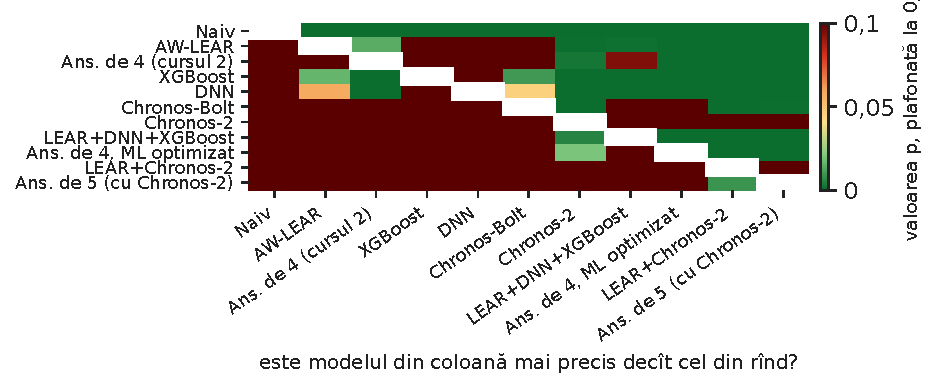
\includegraphics[width=\textwidth,height=0.500\textheight,keepaspectratio]{charts/ro/dm_matrix.pdf}\end{center}\vspace{-3mm}
\chartsource{Sursa: energy-charts.info (Fraunhofer ISE): prețuri OPCOM; consum, producție și fluxuri ENTSO-E; Yahoo Finance (EUA ETC). Date: anul de test 2025-11-01 - 2026-10-31, 365 de zile; valori p unilaterale.}
\vspace{0.5mm}
\begin{itemize}\setlength{\itemsep}{0pt}
  \item AW-LEAR + DNN + XGBoost este mai precis decît AW-LEAR ($p$ = 0{,}001)
    \begin{itemize}\setlength{\itemsep}{0pt}
      \item Cu AW-ARX adăugat, MAE scade la 21{,}69, sub ansamblul din cursul 2 ($p<0{,}001$)
    \end{itemize}
  \item Adăugarea AW-LEAR la Chronos-2 nu schimbă nimic ($p$ = 0{,}491): în zilele dificile, cele două modele greșesc asemănător
\end{itemize}
\par\vfill\noindent{\scriptsize\color{FooterGray}(calcule proprii; teste DM unilaterale)}\hfill\tryit{notebook-ul Jupyter, secțiunea 5}\par\vspace{0.5mm}
\end{frame}

\begin{frame}{Media funcționează pentru că erorile nu sînt identice}
\small
\begin{center}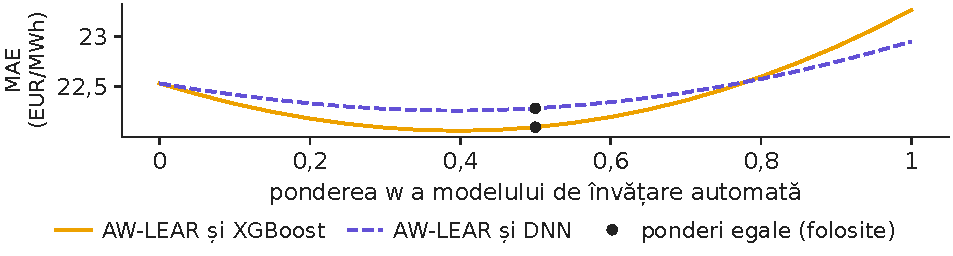
\includegraphics[width=\textwidth,height=0.408\textheight,keepaspectratio]{charts/ro/combo_weight.pdf}\end{center}\vspace{-3mm}
\chartsource{Sursa: energy-charts.info (Fraunhofer ISE): prețuri OPCOM; consum, producție și fluxuri ENTSO-E; Yahoo Finance (EUA ETC). Date: anul de test 2025-11-01 - 2026-10-31; ilustrare, ponderea nu se alege pe anul de test.}
\vspace{0.5mm}
\begin{itemize}\setlength{\itemsep}{0pt}
  \item $\Var\big(\tfrac{e_1+e_2}{2}\big)=\tfrac14(\sigma_1^2+\sigma_2^2+2\rho\sigma_1\sigma_2)$: dacă $\rho<1$, media greșește mai puțin ($e$ = eroarea, $\sigma$ = abaterea ei standard, $\rho$ = corelația)
  \item Corelația erorilor cu AW-LEAR: 0{,}94 (DNN), 0{,}89 (XGBoost)
    \begin{itemize}\setlength{\itemsep}{0pt}
      \item Ponderile egale sînt aproape la fel de bune ca ponderea optimă văzută ulterior (0{,}40)
    \end{itemize}
\end{itemize}
\par\vfill\manager{faceți media cu ponderi egale înainte de a estima ponderi „inteligente”.}\par\vspace{0.5mm}
\par\vfill\noindent{\scriptsize\color{FooterGray}(Bates \& Granger, 1969; calcule proprii)}\hfill\tryit{notebook-ul Jupyter, secțiunea 5}\par\vspace{0.5mm}
\end{frame}

\begin{frame}{Lunar, combinația este mai precisă decît AW-LEAR în 10 din 12 luni}
\small
\begin{center}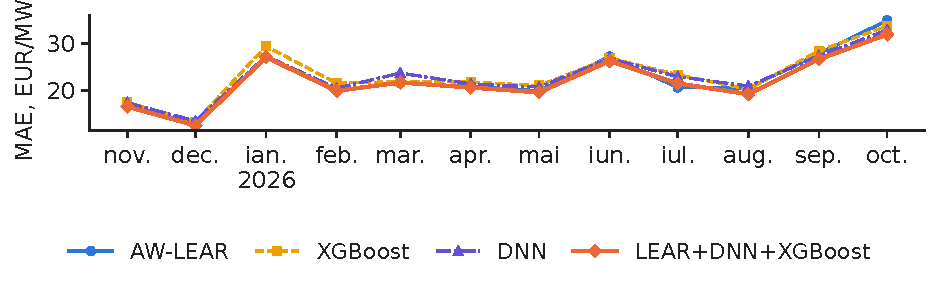
\includegraphics[width=\textwidth,height=0.405\textheight,keepaspectratio]{charts/ro/monthly_ml.pdf}\end{center}\vspace{-3mm}
\chartsource{Sursa: energy-charts.info (Fraunhofer ISE): prețuri OPCOM; consum, producție și fluxuri ENTSO-E; Yahoo Finance (EUA ETC). Date: anul de test 2025-11-01 - 2026-10-31.}
\vspace{0.5mm}
\begin{itemize}\setlength{\itemsep}{0pt}
  \item Luate separat, XGBoost și DNN depășesc AW-LEAR fiecare doar în 3 luni
    \begin{itemize}\setlength{\itemsep}{0pt}
      \item În medie cu acesta, în 10 luni
    \end{itemize}
  \item Toate modelele greșesc mai mult în aceleași luni (ianuarie, iunie, octombrie): zilele dificile sînt dificile pentru toate
\end{itemize}
\par\vfill\manager{raportați comitetului de risc acuratețea lună de lună, nu doar media anuală.}\par\vspace{0.5mm}
\par\vfill\noindent{\scriptsize\color{FooterGray}(calcule proprii, anul de test 1 noiembrie 2025 -- 31 octombrie 2026)}\hfill\tryit{notebook-ul Jupyter, secțiunea 5}\par\vspace{0.5mm}
\end{frame}

\begin{frame}{Costul de calcul: LEAR zilnic este cel mai scump, ML costă minute}
\small
\begin{center}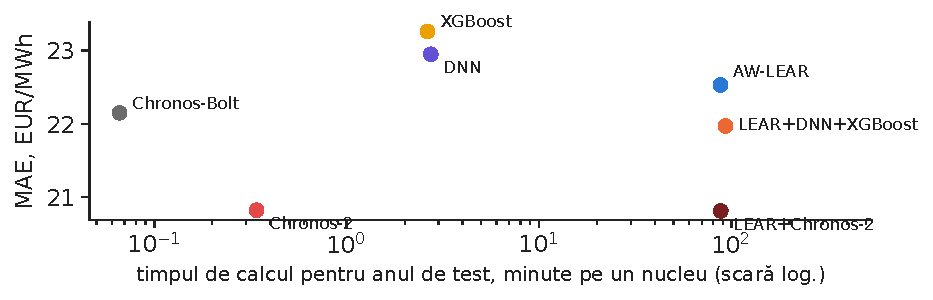
\includegraphics[width=\textwidth,height=0.322\textheight,keepaspectratio]{charts/ro/cost_gain.pdf}\end{center}\vspace{-3mm}
\chartsource{Sursa: energy-charts.info (Fraunhofer ISE): prețuri OPCOM; consum, producție și fluxuri ENTSO-E; Yahoo Finance (EUA ETC). Date: anul de test 2025-11-01 - 2026-10-31; timp măsurat pe un nucleu al calculatorului autorului.}
\vspace{0.5mm}
\begin{itemize}\setlength{\itemsep}{0pt}
  \item Anul de test, pe un nucleu: AW-LEAR 87{,}6 min (365 de zile $\times$ 3 ferestre $\times$ 24 de ore)
    \begin{itemize}\setlength{\itemsep}{0pt}
      \item XGBoost 2{,}6
      \item DNN 2{,}7
      \item Chronos-2 0{,}3
    \end{itemize}
  \item Costuri ascunse: căutarea setărilor (7{,}3 min), preantrenarea Chronos (făcută de alții), oamenii care întrețin fluxul de date
\end{itemize}
\par\vfill\manager{comparați modelele după eroare raportată la costul total de utilizare, nu doar după eroare.}\par\vspace{0.5mm}
\par\vfill\noindent{\scriptsize\color{FooterGray}(calcule proprii; timpi măsurați pe un nucleu al unui laptop cu 18 nuclee)}\hfill\tryit{notebook-ul Jupyter, secțiunea 5}\par\vspace{0.5mm}
\end{frame}


\section{Explicarea prognozelor}

\begin{frame}{Valorile Shapley descompun fiecare prognoză în contribuțiile variabilelor}
\footnotesize
\intuition{Contribuția unei variabile este efectul ei mediu atunci cînd este adăugată în model, calculat pe toate ordinile posibile de adăugare a variabilelor.}
\begin{columns}[T,onlytextwidth]
\begin{column}{0.53\textwidth}
\[ \phi_j=\sum_{S\not\ni j}\tfrac{|S|!\,(p-|S|-1)!}{p!}\big[v(S\cup\{j\})-v(S)\big] \]\vspace{-2mm}\[ \hat f(\mathbf x)=\phi_0+\textstyle\sum_{j}\phi_j \]{\footnotesize\begin{itemize}\setlength{\itemsep}{0pt}
  \item \textbf{\txtwhere}
    \begin{itemize}\setlength{\itemsep}{0pt}
      \item $\phi_j$ = valoarea variabilei $j$ după metoda explicațiilor aditive bazate pe valorile Shapley (SHAP)
      \item $S$ = o submulțime a celorlalte variabile
      \item $v(S)$ = prognoza așteptată cînd se cunoaște doar $S$
      \item $\phi_0$ = prognoza medie
      \item $p$ = 20 de variabile.
    \end{itemize}
\end{itemize}\par}
\end{column}
\begin{column}{0.44\textwidth}
\begin{itemize}\setlength{\itemsep}{1pt}
  \item \textbf{De ce valorile Shapley}
    \begin{itemize}\setlength{\itemsep}{0pt}
      \item Singura împărțire echitabilă în sensul teoriei jocurilor; se adună exact la prognoză
    \end{itemize}
  \item \textbf{Pe datele noastre}
    \begin{itemize}\setlength{\itemsep}{0pt}
      \item XGBoost, 8\,760 de ore de test; cea mai mare diferență dintre $\hat f$ și $\phi_0+\sum\phi_j$: 0{,}000009
      \item Prețurile din zilele anterioare au 69{,}3\% din contribuția totală
    \end{itemize}
\end{itemize}
\end{column}
\end{columns}
\par\vfill\manager{cereți explicația fiecărei alerte, nu doar un clasament global.}\par\vspace{0.5mm}
\par\vfill\noindent{\scriptsize\color{FooterGray}(Shapley, 1953; Lundberg et al., 2020, Nat.\ Mach.\ Intell.)}\hfill\tryit{notebook-ul Jupyter, secțiunea 6}\par\vspace{0.5mm}
\end{frame}

\begin{frame}{Ce determină prognoza arborilor: prețul de ieri, la aceeași oră}
\small
\begin{center}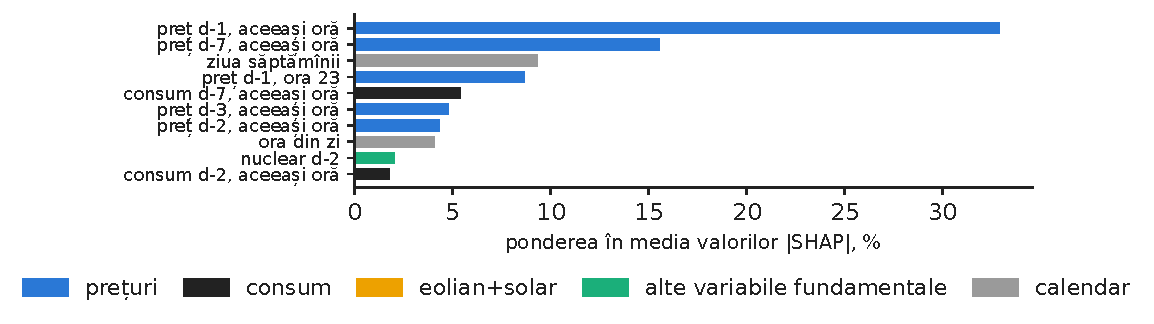
\includegraphics[width=\textwidth,height=0.394\textheight,keepaspectratio]{charts/ro/shap_global.pdf}\end{center}\vspace{-3mm}
\chartsource{Sursa: energy-charts.info (Fraunhofer ISE): prețuri OPCOM; consum, producție și fluxuri ENTSO-E; Yahoo Finance (EUA ETC). Date: anul de test 2025-11-01 - 2026-10-31, 8760 de ore; XGBoost reestimat lunar.}
\vspace{0.5mm}
\begin{itemize}\setlength{\itemsep}{0pt}
  \item Primele variabile: prețul din $d-1$, aceeași oră (32{,}9\%), prețul din $d-7$, aceeași oră (15{,}6\%), ziua săptămînii (9{,}3\%) din media $|\phi|$
  \item Consumul are 8{,}5\%, iar producția eoliană și solară 2{,}5\%: fiind cunoscute doar pînă în $d-2$, sînt informații vechi la închiderea licitației
\end{itemize}
\par\vfill\manager{cumpărați întîi intrări mai bune: prognozele operatorului de transport și de sistem (TSO).}\par\vspace{0.5mm}
\par\vfill\noindent{\scriptsize\color{FooterGray}(calcule proprii, anul de test 1 noiembrie 2025 -- 31 octombrie 2026)}\hfill\tryit{notebook-ul Jupyter, secțiunea 6}\par\vspace{0.5mm}
\end{frame}

\begin{frame}{Producția eoliană și solară scade prețul doar în orele în care este mare}
\small
\begin{center}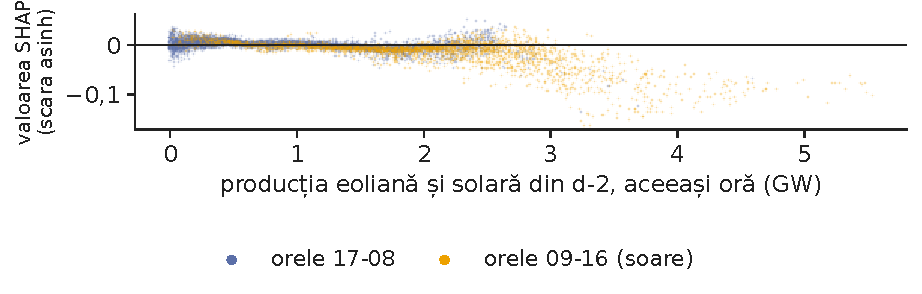
\includegraphics[width=\textwidth,height=0.357\textheight,keepaspectratio]{charts/ro/shap_res.pdf}\end{center}\vspace{-3mm}
\chartsource{Sursa: energy-charts.info (Fraunhofer ISE): prețuri OPCOM; consum, producție și fluxuri ENTSO-E; Yahoo Finance (EUA ETC). Date: anul de test 2025-11-01 - 2026-10-31, 8760 de ore.}
\vspace{0.5mm}
\begin{itemize}\setlength{\itemsep}{0pt}
  \item Fiecare punct este o oră din anul de test: cu cît producția eoliană și solară din $d-2$ la acea oră este mai mare, cu atît contribuția ei este mai negativă (corelație \ensuremath{-}0{,}64)
  \item Efectul apare peste aproximativ 2 gigawați (GW), mai ales la prînz: un prag pe care un model liniar nu îl poate exprima
\end{itemize}
\par\vfill\manager{un dezvoltator de parcuri solare poate citi aici reducerea de preț la care contribuie chiar producția sa.}\par\vspace{0.5mm}
\par\vfill\noindent{\scriptsize\color{FooterGray}(calcule proprii, anul de test 1 noiembrie 2025 -- 31 octombrie 2026)}\hfill\tryit{notebook-ul Jupyter, secțiunea 6}\par\vspace{0.5mm}
\end{frame}

\begin{frame}{Rețeaua neuronală se bazează și mai mult pe prețurile de ieri}
\small
\begin{center}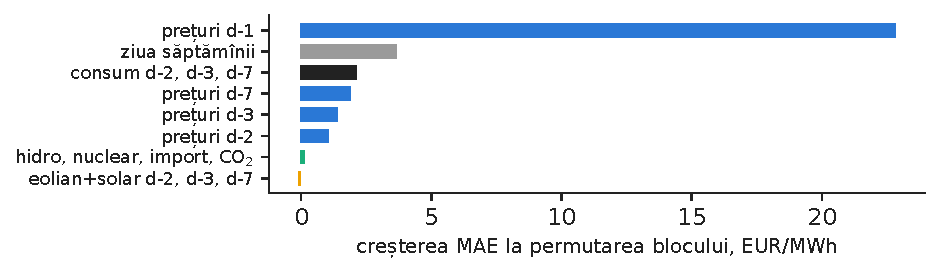
\includegraphics[width=\textwidth,height=0.300\textheight,keepaspectratio]{charts/ro/perm_dnn.pdf}\end{center}\vspace{-3mm}
\chartsource{Sursa: energy-charts.info (Fraunhofer ISE): prețuri OPCOM; consum, producție și fluxuri ENTSO-E; Yahoo Finance (EUA ETC). Date: anul de test 2025-11-01 - 2026-10-31; 5 permutări aleatoare ale zilelor de test.}
\vspace{0.5mm}
\begin{itemize}\setlength{\itemsep}{0pt}
  \item Importanța prin permutare: $I_b$ = MAE cu blocul $b$ amestecat între zilele de test minus MAE fără amestecare (5 permutări)
    \begin{itemize}\setlength{\itemsep}{0pt}
      \item Se aplică oricărui model
    \end{itemize}
  \item Prețurile din $d-1$: +22{,}82 EUR/MWh
    \begin{itemize}\setlength{\itemsep}{0pt}
      \item Ziua săptămînii +3{,}66
      \item Consumul +2{,}12
      \item Producția eoliană și solară \ensuremath{-}0{,}08
    \end{itemize}
\end{itemize}
\par\vfill\manager{monitorizați întîi fluxul prețurilor din $d-1$: fără el, rețeaua cedează.}\par\vspace{0.5mm}
\par\vfill\noindent{\scriptsize\color{FooterGray}(Breiman, 2001, Mach.\ Learn.; calcule proprii)}\hfill\tryit{notebook-ul Jupyter, secțiunea 6}\par\vspace{0.5mm}
\end{frame}


\section{Vîrfuri de preț, prețuri negative și un studiu de caz}

\begin{frame}{Vîrfurile de preț apar seara, prețurile negative la prînz}
\small
\begin{center}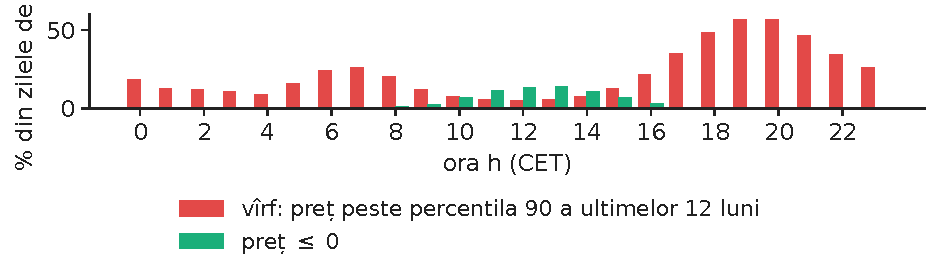
\includegraphics[width=\textwidth,height=0.460\textheight,keepaspectratio]{charts/ro/events_hour.pdf}\end{center}\vspace{-3mm}
\chartsource{Sursa: energy-charts.info (Fraunhofer ISE): prețurile PZU ale OPCOM pentru România. Date: anul de test 2025-11-01 - 2026-10-31.}
\vspace{0.5mm}
\begin{itemize}\setlength{\itemsep}{0pt}
  \item \textbf{Vîrf de preț}: preț peste $\theta$, percentila 90 a prețurilor orare din cele 12 luni dinaintea lunii de livrare
    \begin{itemize}\setlength{\itemsep}{0pt}
      \item $\theta$ între 166{,}8 și 202{,}4 EUR/MWh; 22{,}1\% din orele de test sînt vîrfuri, cele mai multe la ora 19 (57{,}0\% din zile)
    \end{itemize}
  \item \textbf{Preț $\leq$ 0}: 255 de ore, în 53 de zile din anul de test, mai ales în jurul orei 13
\end{itemize}
\par\vfill\manager{o baterie se încarcă la prînz și se descarcă la orele 19--20: cele două evenimente sînt chiar modelul ei de afaceri.}\par\vspace{0.5mm}
\par\vfill\noindent{\scriptsize\color{FooterGray}(calcule proprii, anul de test 1 noiembrie 2025 -- 31 octombrie 2026)}\hfill\tryit{notebook-ul Jupyter, secțiunea 7}\par\vspace{0.5mm}
\end{frame}

\begin{frame}{Clasificarea vîrfurilor: o prognoză bună de preț le detectează deja}
\footnotesize
\intuition{Un clasificator dă probabilitatea ca o oră să fie un vîrf; judecăm cît de bine ordonează orele și cît de corecte sînt probabilitățile lui.}
\begin{columns}[T,onlytextwidth]
\begin{column}{0.56\textwidth}
\[ \hat\pi_{d,h}=\Pr\big(P_{d,h}>\theta_d\mid\mathbf x_{d,h}\big) \]\vspace{-2mm}\[ \text{Brier}=\frac{1}{n}\sum_{d,h}\big(\hat\pi_{d,h}-S_{d,h}\big)^2 \]{\footnotesize\begin{itemize}\setlength{\itemsep}{0pt}
  \item \textbf{\txtwhere}
    \begin{itemize}\setlength{\itemsep}{0pt}
      \item $S_{d,h}$ = 1 dacă ora este un vîrf, 0 altfel
      \item Precizia = ponderea alertelor urmate de vîrfuri
      \item Sensibilitatea = ponderea vîrfurilor semnalate
      \item F1 = media lor armonică
      \item Aria de sub curbă (AUC) = probabilitatea ca o oră cu vîrf să primească un scor mai mare decît o oră obișnuită.
    \end{itemize}
\end{itemize}\par}
\end{column}
\begin{column}{0.41\textwidth}
\begin{itemize}\setlength{\itemsep}{1pt}
  \item \textbf{Pe datele noastre}: clasificatori XGBoost și logistic, reestimați lunar
    \begin{itemize}\setlength{\itemsep}{0pt}
      \item Vîrfuri în 22{,}1\% din orele de test și în 14{,}3\% din ultimul eșantion de antrenare
      \item Scorul Brier: XGBoost 0{,}072; ponderea constantă a vîrfurilor 0{,}172
    \end{itemize}
  \item \textbf{Repere}
    \begin{itemize}\setlength{\itemsep}{0pt}
      \item Persistența: ponderea vîrfurilor la aceeași oră în ultimele 7 zile
      \item Chiar prognoza de preț AW-LEAR, comparată cu $\theta$
    \end{itemize}
\end{itemize}
\end{column}
\end{columns}
\par\vfill\manager{judecați o alertă după probabilitățile ei, nu doar după cîte vîrfuri semnalează.}\par\vspace{0.5mm}
\par\vfill\noindent{\scriptsize\color{FooterGray}(Brier, 1950; Fawcett, 2006)}\hfill\tryit{notebook-ul Jupyter, secțiunea 7}\par\vspace{0.5mm}
\end{frame}

\begin{frame}{Alertele din anul de test: AW-LEAR egalează un clasificator dedicat}
\small
\begin{center}{\footnotesize\renewcommand{\arraystretch}{1.25}\setlength{\tabcolsep}{4pt}
\begin{tabular}{@{}lrrrrrrr@{}}\toprule
Model & AUC & Precizie & Sensibilitate & F1 & Brier & AUC & F1 \\ \midrule
XGBoost & 0{,}953 & 0{,}826 & 0{,}685 & 0{,}749 & 0{,}072 & 0{,}980 & 0{,}571 \\
Regresie logistică & 0{,}953 & 0{,}847 & 0{,}641 & 0{,}730 & 0{,}072 & 0{,}980 & 0{,}581 \\
Persistență, 7 zile & 0{,}918 & 0{,}761 & 0{,}681 & 0{,}719 & 0{,}083 & 0{,}847 & 0{,}205 \\
Prognoza AW-LEAR $>\theta$ & 0{,}959 & 0{,}851 & 0{,}733 & 0{,}788 & -- & 0{,}983 & 0{,}558 \\
\bottomrule\end{tabular}}\end{center}
\par\vspace{0.5mm}{\scriptsize \begin{itemize}\setlength{\itemsep}{0pt}
  \item Coloanele 2--6: vîrfuri (1\,938 de ore); coloanele 7--8: prețuri $\leq$ 0 (255 de ore). Alertă cînd probabilitatea $>$ 0{,}5; AW-LEAR: alertă cînd prognoza prețului depășește $\theta$ (sau este $\leq$ 0).
  \item La prețurile negative, XGBoost semnalează doar o fracțiune 0{,}467 din evenimente la pragul 0{,}5: aceste ore sînt rare și depind de vremea de mîine.
\end{itemize}}
\par\vfill\manager{cumpărați un serviciu de alertă pentru vîrfuri doar dacă depășește semnalul ascuns deja în prognoza dumneavoastră de preț.}\par\vspace{0.5mm}
\par\vfill\noindent{\scriptsize\color{FooterGray}(calcule proprii, anul de test 1 noiembrie 2025 -- 31 octombrie 2026)}\hfill\tryit{notebook-ul Jupyter, secțiunea 7}\par\vspace{0.5mm}
\end{frame}

\begin{frame}{Persistența detectează vîrfurile, dar nu și prețurile negative}
\small
\begin{center}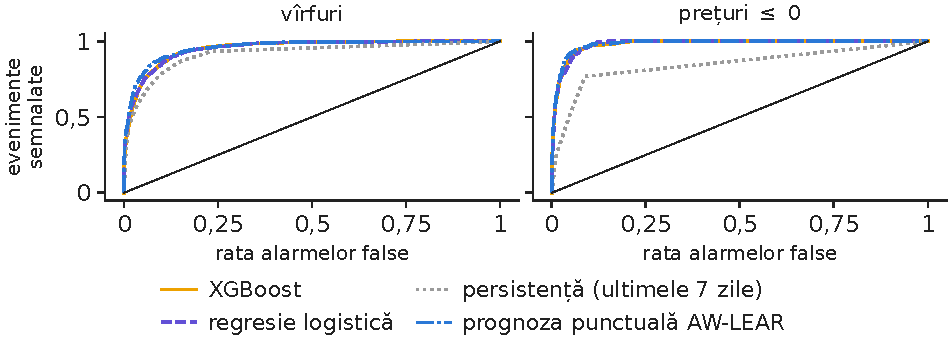
\includegraphics[width=\textwidth,height=0.480\textheight,keepaspectratio]{charts/ro/roc.pdf}\end{center}\vspace{-3mm}
\chartsource{Sursa: energy-charts.info (Fraunhofer ISE): prețuri OPCOM; consum, producție și fluxuri ENTSO-E; Yahoo Finance (EUA ETC). Date: anul de test 2025-11-01 - 2026-10-31, 8760 de ore.}
\vspace{0.5mm}
\begin{itemize}\setlength{\itemsep}{0pt}
  \item Curbele caracteristice de operare (ROC)
    \begin{itemize}\setlength{\itemsep}{0pt}
      \item Vîrfuri: AUC între 0{,}918 (persistență) și 0{,}959 (AW-LEAR), deoarece vîrful de seară se repetă de la o zi la alta
    \end{itemize}
  \item Prețuri negative: persistența are AUC 0{,}847, față de 0{,}980 pentru XGBoost
    \begin{itemize}\setlength{\itemsep}{0pt}
      \item Ele depind de soarele și vîntul de mîine, nu de ziua de ieri
    \end{itemize}
\end{itemize}
\par\vfill\noindent{\scriptsize\color{FooterGray}(calcule proprii, anul de test 1 noiembrie 2025 -- 31 octombrie 2026)}\hfill\tryit{notebook-ul Jupyter, secțiunea 7}\par\vspace{0.5mm}
\end{frame}

\begin{frame}{Regula cost--pierdere: reacționați cînd probabilitatea depășește C/L}
\small
\begin{center}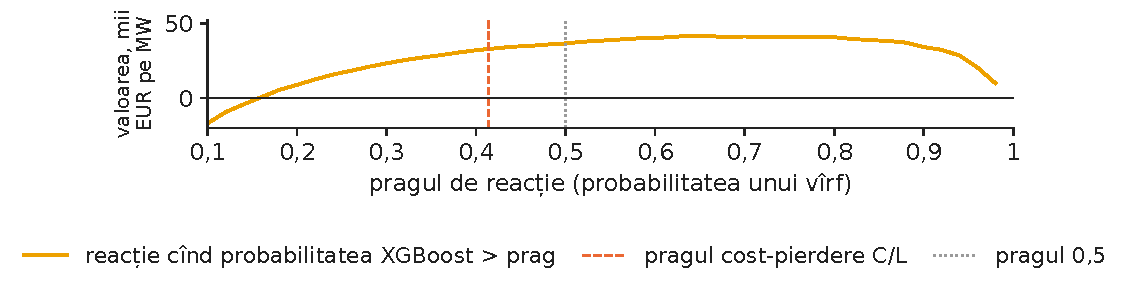
\includegraphics[width=\textwidth,height=0.340\textheight,keepaspectratio]{charts/ro/decision.pdf}\end{center}\vspace{-3mm}
\chartsource{Sursa: energy-charts.info (Fraunhofer ISE): prețuri OPCOM; consum, producție și fluxuri ENTSO-E; Yahoo Finance (EUA ETC). Date: anul de test 2025-11-01 - 2026-10-31; 1 MW de consum flexibil, C = 30 EUR/MWh (ipoteză).}
\vspace{0.5mm}
\begin{itemize}\setlength{\itemsep}{0pt}
  \item \textbf{Regula}: reacție dacă $\hat\pi_{d,h}>C/\bar L$ = 30/72{,}5 = 0{,}414; C = costul reacției, $\bar L$ = costul unui vîrf ratat
    \begin{itemize}\setlength{\itemsep}{0pt}
      \item Mutarea a 1 MWh dintr-o oră cu alertă aduce $P_{d,h}-\theta_d-C$; C = 30 EUR/MWh (ipoteză); $\bar L$ = depășirea medie a pragului în anul de validare
    \end{itemize}
  \item Valoarea pe MW și an: 33{,}0 mii EUR la pragul C/L, 11{,}8 cu persistența, 62{,}4 cu informație perfectă
\end{itemize}
\par\vfill\manager{stabiliți pragul din propriile costuri
    \begin{itemize}\setlength{\itemsep}{0pt}
      \item Cel mai bun prag văzut ulterior (0{,}64) este înțelepciune retrospectivă.
    \end{itemize}}\par\vspace{0.5mm}
\par\vfill\noindent{\scriptsize\color{FooterGray}(Murphy, 1977, MWR; calcule proprii)}\hfill\tryit{notebook-ul Jupyter, secțiunea 7}\par\vspace{0.5mm}
\end{frame}

\begin{frame}{Studiu de caz, 30 iunie 2026: vîrful a fost anticipat, amploarea lui nu}
\small
\begin{center}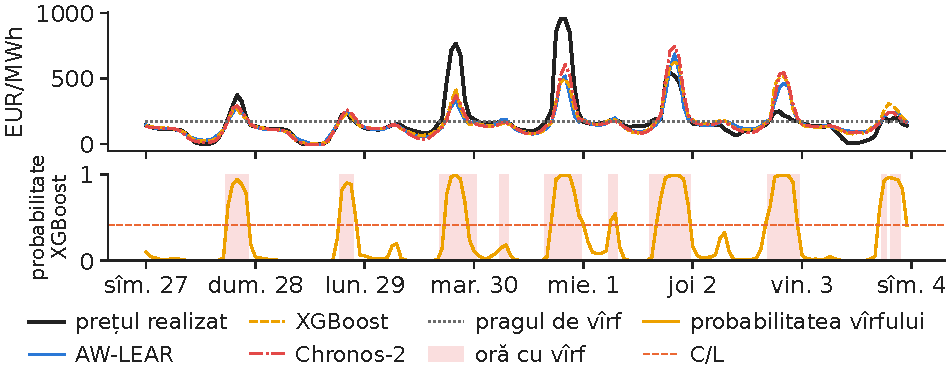
\includegraphics[width=\textwidth,height=0.417\textheight,keepaspectratio]{charts/ro/case_week.pdf}\end{center}\vspace{-3mm}
\chartsource{Sursa: energy-charts.info (Fraunhofer ISE): prețuri OPCOM; consum, producție și fluxuri ENTSO-E; Yahoo Finance (EUA ETC). Date: 2026-06-27 - 2026-07-03, date orare.}
\vspace{0.5mm}
\begin{itemize}\setlength{\itemsep}{0pt}
  \item \textbf{Ora 20:00 CET}: 954{,}59 EUR/MWh, cel mai mare preț din anul de test
    \begin{itemize}\setlength{\itemsep}{0pt}
      \item Prognoze: AW-LEAR 520, XGBoost 499, DNN 614, Chronos-2 607; probabilitatea vîrfului 0{,}992
    \end{itemize}
  \item Săptămîna 27 iunie 2026 -- 3 iulie 2026: 47 de ore cu vîrfuri, 45 de alerte la pragul C/L, iar 39 de alerte au fost corecte
\end{itemize}
\par\vfill\manager{probabilitatea arată dacă reacționați, prognoza punctuală arată cît.}\par\vspace{0.5mm}
\par\vfill\noindent{\scriptsize\color{FooterGray}(calcule proprii; prețurile PZU din România)}\hfill\tryit{notebook-ul Jupyter, secțiunea 8}\par\vspace{0.5mm}
\end{frame}

\begin{frame}{Studiu de caz: arborii au urmat seara extremă din ziua precedentă}
\small
\begin{center}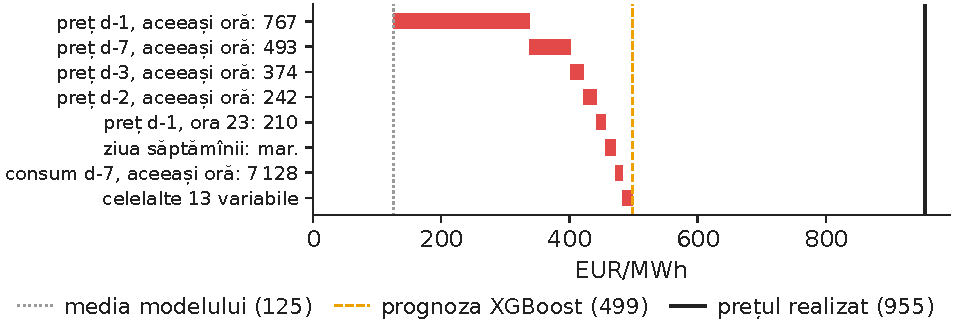
\includegraphics[width=\textwidth,height=0.457\textheight,keepaspectratio]{charts/ro/shap_local.pdf}\end{center}\vspace{-3mm}
\chartsource{Sursa: energy-charts.info (Fraunhofer ISE): prețuri OPCOM; consum, producție și fluxuri ENTSO-E; Yahoo Finance (EUA ETC). Date: 2026-06-30, ora 20:00 CET; contribuții exprimate în EUR/MWh (anexa C).}
\vspace{0.5mm}
\begin{itemize}\setlength{\itemsep}{0pt}
  \item De la 125 (prognoza medie) la 499 EUR/MWh: prețul din $d-1$, aceeași oră, \ensuremath{+}213
    \begin{itemize}\setlength{\itemsep}{0pt}
      \item Prețul din $d-7$ \ensuremath{+}64
    \end{itemize}
  \item Arborii nu pot depăși prețurile memorate în frunze: valorile extreme sînt plafonate
\end{itemize}
\par\vfill\manager{prezentați consiliului de administrație această descompunere pentru fiecare alertă importantă.}\par\vspace{0.5mm}
\par\vfill\noindent{\scriptsize\color{FooterGray}(calcule proprii; valori SHAP în EUR/MWh, anexa C)}\hfill\tryit{notebook-ul Jupyter, secțiunea 8}\par\vspace{0.5mm}
\end{frame}

\begin{frame}{Avertizarea timpurie a vîrfurilor: lucrarea grupului și replicarea ei}
\footnotesize
\begin{itemize}\setlength{\itemsep}{1pt}
  \item \textbf{Ce a făcut lucrarea} (Andrei, Pele, Cramer, Amza \& Diaconu, 2026)
    \begin{itemize}\setlength{\itemsep}{0pt}
      \item Date: 5.000 de ore de pe PZU din România, în 2024, cu date despre consum, surse regenerabile și combustibili; vîrf = preț peste percentila 90
      \item Metodă: păduri aleatoare și XGBoost, explicate cu SHAP; un scor de avertizare construit din pragurile mai multor indicatori
      \item Rezultat: prețul anterior și prognoza consumului rezidual sînt principalii factori ai vîrfurilor
    \end{itemize}
  \item \textbf{Replicarea noastră} (studiul de caz C7, numai cu informația de la închiderea licitației)
    \begin{itemize}\setlength{\itemsep}{0pt}
      \item Perioada de test: iulie 2025 -- octombrie 2026; vîrfuri în 22{,}1\% din ore (în antrenare: 10{,}0\%)
      \item XGBoost: AUC 0{,}946; principalii factori: prețul de ieri și cel de acum o săptămînă, la aceeași oră, ca pe diapozitivele anterioare
    \end{itemize}
\end{itemize}
\par\vspace{0.5mm}{\scriptsize \begin{itemize}\setlength{\itemsep}{0pt}
  \item Rezultatele lucrării sînt cele raportate de autori; cifrele replicării sînt calculate cu notebook-ul Jupyter al studiului de caz C7, pe datele noastre.
\end{itemize}}
\par\vfill\manager{prognoza consumului rezidual este variabila de care un model de vîrfuri are cea mai mare nevoie și care lipsește din datele noastre publice.}\par\vspace{0.5mm}
\par\vfill\noindent{\scriptsize\color{FooterGray}(Andrei, Pele, Cramer, Amza \& Diaconu, 2026, PICBE; studiul de caz C7)}\par\vspace{0.5mm}
\end{frame}


\section{Capcane care fac un model să pară mai bun}

\begin{frame}{Informația din viitor: două evaluări invalide avantajează XGBoost}
\small
\begin{center}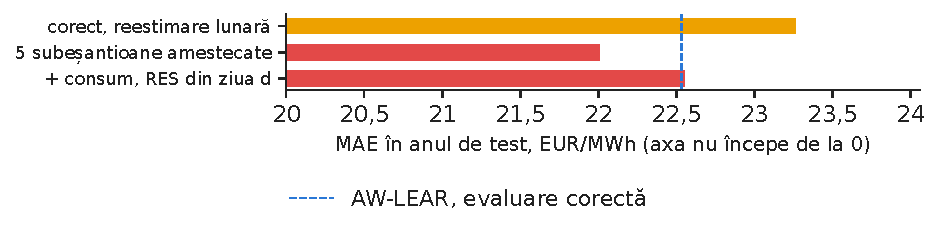
\includegraphics[width=\textwidth,height=0.337\textheight,keepaspectratio]{charts/ro/pit_leak.pdf}\end{center}\vspace{-3mm}
\chartsource{Sursa: energy-charts.info (Fraunhofer ISE): prețuri OPCOM; consum, producție și fluxuri ENTSO-E; Yahoo Finance (EUA ETC). Date: anul de test 2025-11-01 - 2026-10-31; XGBoost, configurația aleasă.}
\vspace{0.5mm}
\begin{itemize}\setlength{\itemsep}{0pt}
  \item \textbf{Validare încrucișată cu 5 subeșantioane amestecate}: zile din viitor ajung în eșantionul de antrenare
    \begin{itemize}\setlength{\itemsep}{0pt}
      \item MAE 22{,}01 în loc de 23{,}26: cu 5{,}4\% mai bine, doar pe hîrtie
    \end{itemize}
  \item \textbf{Consumul și producția eoliană și solară din ziua $d$ ca intrări}: nu sînt cunoscute la ora 12:00 în ziua $d-1$; în grafic, surse regenerabile de energie (RES)
    \begin{itemize}\setlength{\itemsep}{0pt}
      \item MAE 22{,}55; un cîștig aparent de 3{,}1\%, cel mult cît ar putea aduce prognoze perfecte ale acestor variabile
    \end{itemize}
\end{itemize}
\par\vfill\manager{cereți oricărui furnizor o testare cronologică, cu fiecare intrare datată la momentul închiderii licitației.}\par\vspace{0.5mm}
\par\vfill\noindent{\scriptsize\color{FooterGray}(Bergmeir \& Benítez, 2012, Inf.\ Sci.; calcule proprii)}\hfill\tryit{notebook-ul Jupyter, secțiunea 9}\par\vspace{0.5mm}
\end{frame}

\begin{frame}{Alegerea pe anul de test simulează o victorie asupra LEAR}
\small
\begin{center}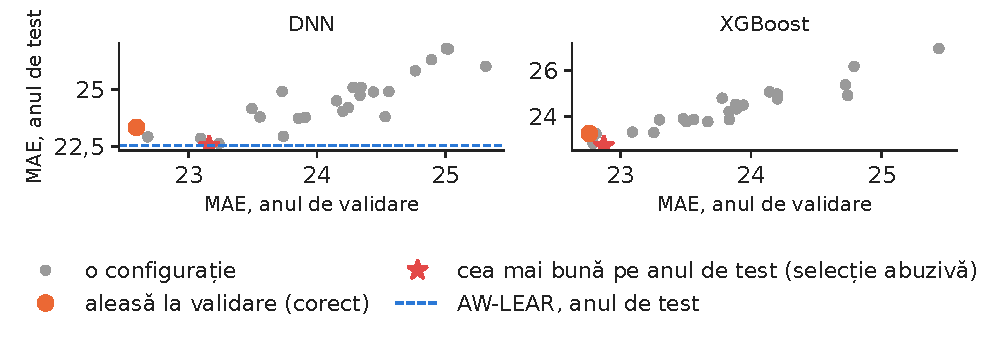
\includegraphics[width=\textwidth,height=0.345\textheight,keepaspectratio]{charts/ro/snooping.pdf}\end{center}\vspace{-3mm}
\chartsource{Sursa: energy-charts.info (Fraunhofer ISE): prețuri OPCOM; consum, producție și fluxuri ENTSO-E; Yahoo Finance (EUA ETC). Date: anul de validare și anul de test 2025-11-01 - 2026-10-31; o inițializare pe configurație.}
\vspace{0.5mm}
\begin{itemize}\setlength{\itemsep}{0pt}
  \item Rețeaua DNN aleasă corect (la validare, o inițializare): MAE 23{,}34
    \begin{itemize}\setlength{\itemsep}{0pt}
      \item Cea mai bună dintre cele 25 de setări pe anul de test: 22{,}52, chiar sub AW-LEAR (22{,}53)
    \end{itemize}
  \item Clasamentele de validare și de test sînt apropiate (corelația Spearman 0{,}86 pentru DNN, 0{,}94 pentru XGBoost): validarea funcționează, dar nu este perfectă
\end{itemize}
\par\vfill\manager{întrebați cîte modele au fost încercate înaintea celui prezentat
    \begin{itemize}\setlength{\itemsep}{0pt}
      \item Cu cît sînt mai multe încercări, cu atît cel mai bun pare mai bun decît este.
    \end{itemize}}\par\vspace{0.5mm}
\par\vfill\noindent{\scriptsize\color{FooterGray}(White, 2000, Econometrica; calcule proprii)}\hfill\tryit{notebook-ul Jupyter, secțiunea 9}\par\vspace{0.5mm}
\end{frame}

\begin{frame}{Reestimarea: un model neactualizat un an pierde 4{,}3\%}
\small
\begin{center}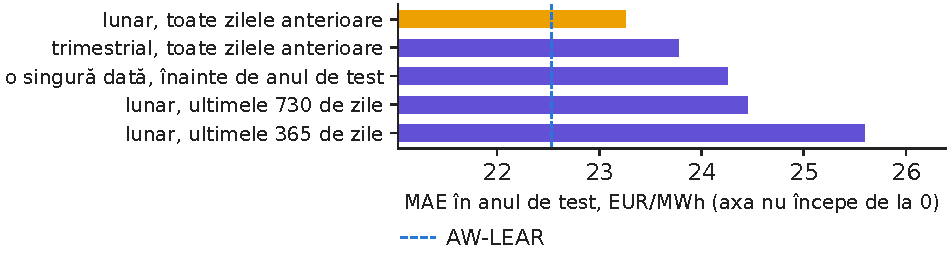
\includegraphics[width=\textwidth,height=0.401\textheight,keepaspectratio]{charts/ro/pit_retrain.pdf}\end{center}\vspace{-3mm}
\chartsource{Sursa: energy-charts.info (Fraunhofer ISE): prețuri OPCOM; consum, producție și fluxuri ENTSO-E; Yahoo Finance (EUA ETC). Date: anul de test 2025-11-01 - 2026-10-31; XGBoost, configurația aleasă.}
\vspace{0.5mm}
\begin{itemize}\setlength{\itemsep}{0pt}
  \item Estimat o singură dată, înaintea anului de test: MAE 24{,}25
    \begin{itemize}\setlength{\itemsep}{0pt}
      \item Pierderea crește în timp (+0{,}15 EUR/MWh în primele 3 luni, +3{,}70 în ultimele 3)
    \end{itemize}
  \item O fereastră glisantă scurtă (365 de zile, MAE 25{,}59) este mai slabă decît întregul istoric: arborii au nevoie de multe vîrfuri din trecut pentru a învăța
\end{itemize}
\par\vfill\manager{includeți reestimarea lunară în calendarul operațional, cu un responsabil, ca pe orice alt control.}\par\vspace{0.5mm}
\par\vfill\noindent{\scriptsize\color{FooterGray}(calcule proprii, anul de test 1 noiembrie 2025 -- 31 octombrie 2026)}\hfill\tryit{notebook-ul Jupyter, secțiunea 9}\par\vspace{0.5mm}
\end{frame}

\begin{frame}{Testul de scurgere a informației: ștergerea viitorului nu schimbă nimic}
\footnotesize
\begin{columns}[T,onlytextwidth]
\begin{column}{0.52\textwidth}
\begin{itemize}\setlength{\itemsep}{1pt}
  \item \textbf{Testul}
    \begin{itemize}\setlength{\itemsep}{0pt}
      \item Pentru prima zi din fiecare dintre cele 12 luni de test, toate datele de după ora 12:00 din ziua $d-1$ sînt șterse, apoi înlocuite cu 10\,000 EUR/MWh
      \item XGBoost, rețeaua DNN și clasificatorul de vîrfuri sînt reestimate și trebuie să dea aceleași prognoze
    \end{itemize}
  \item \textbf{Rezultatul}
    \begin{itemize}\setlength{\itemsep}{0pt}
      \item Arborii și clasificatorul: prognoze identice; DNN: diferențe sub 0{,}001 EUR/MWh (rotunjiri ale calculelor paralele)
      \item Chronos: contextul este construit numai din zilele dinaintea zilei $d$, verificat în cod
    \end{itemize}
\end{itemize}
\end{column}
\begin{column}{0.45\textwidth}
\begin{itemize}\setlength{\itemsep}{1pt}
  \item \textbf{Lista de verificare înainte de a avea încredere într-un model}
    \begin{itemize}\setlength{\itemsep}{0pt}
      \item Fiecare intrare datată la momentul închiderii licitației
      \item Setări alese pe un an de validare
      \item Un singur an de test, deschis o singură dată, cu teste DM față de LEAR
      \item Reestimări lunare și un test de perturbare ca acesta
    \end{itemize}
\end{itemize}
\end{column}
\end{columns}
\par\vfill\manager{includeți această verificare în evaluarea oricărui model, statistic sau de învățare automată.}\par\vspace{0.5mm}
\par\vfill\noindent{\scriptsize\color{FooterGray}(cursul 2; Lago et al., 2021, APEN)}\hfill\tryit{notebook-ul Jupyter, secțiunea 10}\par\vspace{0.5mm}
\end{frame}

\section*{Recapitulare}

\begin{frame}{Test 1: o testare retrospectivă perfectă}
\small
\begin{itemize}
  \item Un start-up prezintă o rețea neuronală cu rMAE 0{,}70 pentru România, testată prin validare încrucișată cu 5 subeșantioane amestecate
    \begin{itemize}\setlength{\itemsep}{0pt}
      \item Ce cereți?
    \end{itemize}
\end{itemize}
\vspace{2mm}
\begin{exampleblock}{R\u{a}spuns}
\begin{itemize}
  \item O testare cronologică pe un an neatins, cu intrări cunoscute la ora 12:00 în ziua $d-1$: pe datele noastre, doar amestecarea a făcut XGBoost să pară cu 5{,}4\% mai bun.
\end{itemize}
\end{exampleblock}
\end{frame}

\begin{frame}{Test 2: ce model puneți în producție}
\small
\begin{itemize}
  \item Chronos-2 are cea mai mică MAE dintre modelele individuale
    \begin{itemize}\setlength{\itemsep}{0pt}
      \item Combinația AW-LEAR + Chronos-2 are aceeași MAE
      \item Pe care o puneți în producție?
    \end{itemize}
\end{itemize}
\vspace{2mm}
\begin{exampleblock}{R\u{a}spuns}
\begin{itemize}
  \item Combinația: aceeași acuratețe (DM, $p$ = 0{,}491), dar dacă modelul preantrenat se degradează sau devine indisponibil, LEAR asigură în continuare jumătate din prognoză.
\end{itemize}
\end{exampleblock}
\end{frame}

\begin{frame}{Test 3: interpretarea valorilor SHAP}
\small
\begin{itemize}
  \item Consumul are o pondere SHAP mică (8{,}5\%)
    \begin{itemize}\setlength{\itemsep}{0pt}
      \item Putem concluziona că acesta nu influențează prețul?
    \end{itemize}
\end{itemize}
\vspace{2mm}
\begin{exampleblock}{R\u{a}spuns}
\begin{itemize}
  \item Nu: SHAP explică modelul, nu piața
    \begin{itemize}\setlength{\itemsep}{0pt}
      \item Consumul intră doar cu valoarea din ziua $d-2$, deja reflectată în prețul de ieri.
    \end{itemize}
\end{itemize}
\end{exampleblock}
\end{frame}

\begin{frame}{Test 4: pragul de alertă}
\small
\begin{itemize}
  \item Mutarea a 1 MWh vă costă 60 EUR în loc de 30
    \begin{itemize}\setlength{\itemsep}{0pt}
      \item Cum se schimbă pragul de alertă?
    \end{itemize}
\end{itemize}
\vspace{2mm}
\begin{exampleblock}{R\u{a}spuns}
\begin{itemize}
  \item Se dublează: C/L crește de la 0{,}414 la aproximativ dublul acestei valori, deci reacționați numai la vîrfurile mai sigure.
\end{itemize}
\end{exampleblock}
\end{frame}

\begin{frame}{Test 5: reestimarea}
\small
\begin{itemize}
  \item Echipa de date propune ca modelul să fie antrenat o dată pe an, pentru a economisi efort
    \begin{itemize}\setlength{\itemsep}{0pt}
      \item Ce arată anul de test?
    \end{itemize}
\end{itemize}
\vspace{2mm}
\begin{exampleblock}{R\u{a}spuns}
\begin{itemize}
  \item Un model neactualizat un an a fost cu 4{,}3\% mai puțin precis, iar diferența a crescut în ultimele luni
    \begin{itemize}\setlength{\itemsep}{0pt}
      \item O reestimare lunară a XGBoost durează circa 13 de secunde.
    \end{itemize}
\end{itemize}
\end{exampleblock}
\end{frame}

\begin{frame}{Recapitulare}
\small
\vspace{-2mm}\begin{multicols}{2}\scriptsize\tableofcontents\end{multicols}
\begin{itemize}\setlength{\itemsep}{1pt}
  \item Calibrate, rețeaua DNN și XGBoost sînt mai precise decît în cursul 2, dar nu depășesc singure AW-LEAR
    \begin{itemize}\setlength{\itemsep}{0pt}
      \item În medie cu acesta, îl depășesc
    \end{itemize}
  \item Chronos-2, fără antrenare, este cel mai precis model individual (MAE 20{,}82, cu 7{,}6\% sub AW-LEAR)
    \begin{itemize}\setlength{\itemsep}{0pt}
      \item Orice model trebuie explicat, validat și reestimat
    \end{itemize}
\end{itemize}
\end{frame}

\begin{frame}{Cercetările grupului nostru: învățarea automată pe piața din România}
\footnotesize
\begin{itemize}\setlength{\itemsep}{1pt}
  \item \textbf{Avertizarea timpurie a vîrfurilor de preț} (Andrei, Pele, Cramer, Amza \& Diaconu, 2026, PICBE)
    \begin{itemize}\setlength{\itemsep}{0pt}
      \item Ce a făcut lucrarea: a construit un sistem explicabil de inteligență artificială (AI) pentru PZU din România
      \item Rezultat: prețul anterior și consumul rezidual sînt principalii factori ai vîrfurilor (studiul de caz C7)
    \end{itemize}
  \item \textbf{Explicarea prognozelor de preț pe mai multe orizonturi} (Andrei, Pele \& Cramer, 2026, PICBE)
    \begin{itemize}\setlength{\itemsep}{0pt}
      \item Ce a făcut lucrarea: a explicat prognozele de învățare automată pentru prețurile orare din România
      \item Rezultat: arată ce factori contează la fiecare orizont și în fiecare regim de preț
    \end{itemize}
  \item \textbf{Patru generații de modele pentru prețul energiei} (Andrei, Velev, Toma, Pele \& Lessmann, 2024, arXiv 2411.03372)
    \begin{itemize}\setlength{\itemsep}{0pt}
      \item Ce a făcut lucrarea: a comparat patru generații de metode de prognoză a prețurilor energiei, de la modelele statistice la învățarea profundă
      \item Utilitate: un reper pentru alegerea familiei de modele
    \end{itemize}
  \item \textbf{Modele fundaționale pentru riscul extrem} (Jheng, Tak, Găman, Mazurencu-Marinescu-Pele \& Pele, 2026, ECECSR)
    \begin{itemize}\setlength{\itemsep}{0pt}
      \item Ce a făcut lucrarea: a folosit modele fundaționale preantrenate, fără reantrenare și cu calibrare conformală, pentru prognoza pierderilor extreme pe piețele din Europa Centrală și de Est
    \end{itemize}
\end{itemize}
\par\vspace{0.5mm}{\scriptsize \begin{itemize}\setlength{\itemsep}{0pt}
  \item Rezultatele de pe acest diapozitiv sînt cele raportate în lucrări; celelalte cifre din curs provin din calculele noastre.
\end{itemize}}
\par\vfill\noindent{\scriptsize\color{FooterGray}(Academia de Studii Economice din București; Academia Română, Institutul de Prognoză Economică)}\par\vspace{0.5mm}
\end{frame}

\begin{frame}{Lecturi și resurse suplimentare}
\small
\begin{columns}[T,onlytextwidth]
\begin{column}{0.52\textwidth}
\begin{itemize}\setlength{\itemsep}{1pt}
  \item \textbf{epftoolbox}: rețeaua DNN și modelul LEAR din Lago et al.\ (2021), cu date deschise pentru evaluare --- \href{https://github.com/jeslago/epftoolbox}{github.com/jeslago/epftoolbox}.
  \item \textbf{XGBoost} și \textbf{shap}, documentație: \href{https://xgboost.readthedocs.io}{xgboost.readthedocs.io}, \href{https://shap.readthedocs.io}{shap.readthedocs.io}.
  \item \textbf{Chronos}, modele fundaționale: \href{https://github.com/amazon-science/chronos-forecasting}{github.com/amazon-science/chronos-forecasting}.
  \item \textbf{Interpretable Machine Learning} (C.\ Molnar), gratuit online: \href{https://christophm.github.io/interpretable-ml-book/}{christophm.github.io}.
\end{itemize}
\end{column}
\begin{column}{0.45\textwidth}
\begin{itemize}\setlength{\itemsep}{1pt}
  \item \textbf{Acest curs}: cod, date, notebook-uri Jupyter --- \href{https://github.com/danpele/EMQA}{github.com/danpele/EMQA}.
  \item \textbf{Studiul de caz C7} replică pe datele cursului lucrarea despre avertizarea timpurie a vîrfurilor.
  \item \textbf{Exercițiu practic}: notebook-ul Jupyter reproduce toate graficele și cifrele din acest curs --- \href{\emqarepo/\emqanb}{notebooks/}.
\end{itemize}
\end{column}
\end{columns}
\end{frame}

\begin{frame}{Bibliografie (1/3)}
\scriptsize
\begin{itemize}\setlength{\itemsep}{1pt}\scriptsize
\item Andrei, A.-V., Pele, D.-T.\ \& Cramer, A.-A.\ (2026). Multi-horizon explainability in energy price forecasting: Disentangling market dynamics and renewable intermittency in Romania's liberalized electricity market. \textit{Proceedings of the International Conference on Business Excellence}, 20(1), 104--117. \href{https://doi.org/10.2478/picbe-2026-0014}{doi:10.2478/picbe-2026-0014}
\item Andrei, A.-V., Pele, D.-T., Cramer, A.-A., Amza, A.\ \& Diaconu, D.\ (2026). Explainable AI-based early warning system for electricity price spikes: Evidence from the Romanian market. \textit{Proceedings of the International Conference on Business Excellence}, 20(1), 4820--4836. \href{https://doi.org/10.2478/picbe-2026-0352}{doi:10.2478/picbe-2026-0352}
\item Andrei, A.-V., Velev, G., Toma, F.-M., Pele, D.\,T.\ \& Lessmann, S.\ (2024). Energy price modelling: A comparative evaluation of four generations of forecasting methods. arXiv:2411.03372.
\item Ansari, A.\,F., Stella, L., Turkmen, C.\ et al.\ (2024). Chronos: Learning the language of time series. \textit{Transactions on Machine Learning Research}. arXiv:2403.07815.
\item Ansari, A.\,F., Shchur, O., Küken, J.\ et al.\ (2025). Chronos-2: From univariate to universal forecasting. arXiv:2510.15821.
\item Bates, J.\,M.\ \& Granger, C.\,W.\,J.\ (1969). The combination of forecasts. \textit{Journal of the Operational Research Society}, 20(4), 451--468. \href{https://doi.org/10.1057/jors.1969.103}{doi:10.1057/jors.1969.103}
\item Bergmeir, C.\ \& Benítez, J.\,M.\ (2012). On the use of cross-validation for time series predictor evaluation. \textit{Information Sciences}, 191, 192--213. \href{https://doi.org/10.1016/j.ins.2011.12.028}{doi:10.1016/j.ins.2011.12.028}
\item Bergstra, J.\ \& Bengio, Y.\ (2012). Random search for hyper-parameter optimization. \textit{Journal of Machine Learning Research}, 13, 281--305.
\item Breiman, L.\ (2001). Random forests. \textit{Machine Learning}, 45(1), 5--32. \href{https://doi.org/10.1023/A:1010933404324}{doi:10.1023/A:1010933404324}
\end{itemize}
\end{frame}

\begin{frame}{Bibliografie (2/3)}
\scriptsize
\begin{itemize}\setlength{\itemsep}{1pt}\scriptsize
\item Brier, G.\,W.\ (1950). Verification of forecasts expressed in terms of probability. \textit{Monthly Weather Review}, 78(1), 1--3. \href{https://doi.org/10.1175/1520-0493(1950)078<0001:VOFEIT>2.0.CO;2}{doi:10.1175/1520-0493(1950)078\allowbreak<0001:VOFEIT>2.0.CO;2}
\item Chen, T.\ \& Guestrin, C.\ (2016). XGBoost: A scalable tree boosting system. \textit{Proceedings of the 22nd ACM SIGKDD Conference}, 785--794. \href{https://doi.org/10.1145/2939672.2939785}{doi:10.1145/2939672.2939785}
\item Diebold, F.\,X.\ \& Mariano, R.\,S.\ (1995). Comparing predictive accuracy. \textit{Journal of Business \& Economic Statistics}, 13(3), 253--263. \href{https://doi.org/10.1080/07350015.1995.10524599}{doi:10.1080/07350015.1995.10524599}
\item Fawcett, T.\ (2006). An introduction to ROC analysis. \textit{Pattern Recognition Letters}, 27(8), 861--874. \href{https://doi.org/10.1016/j.patrec.2005.10.010}{doi:10.1016/j.patrec.2005.10.010}
\item Friedman, J.\,H.\ (2001). Greedy function approximation: A gradient boosting machine. \textit{Annals of Statistics}, 29(5), 1189--1232. \href{https://doi.org/10.1214/aos/1013203451}{doi:10.1214/aos/1013203451}
\item Hastie, T., Tibshirani, R.\ \& Friedman, J.\ (2009). \textit{The Elements of Statistical Learning}, 2nd ed. Springer. \href{https://doi.org/10.1007/978-0-387-84858-7}{doi:10.1007/978-0-387-84858-7}
\item Jheng, S., Tak, R., Găman, Ș., Mazurencu-Marinescu-Pele, M.\ \& Pele, D.\,T.\ (2026). Can foundation models manage risk? Zero-shot VaR and ES forecasting with conformal calibration in CEE markets. \textit{Economic Computation and Economic Cybernetics Studies and Research}, 60(2), 267--290. \href{https://doi.org/10.24818/18423264/60.2.26.14}{doi:10.24818/18423264/60.2.26.14}
\item Kingma, D.\,P.\ \& Ba, J.\ (2015). Adam: A method for stochastic optimization. \textit{International Conference on Learning Representations}. arXiv:1412.6980.
\item Lago, J., De Ridder, F.\ \& De Schutter, B.\ (2018). Forecasting spot electricity prices: Deep learning approaches and empirical comparison of traditional algorithms. \textit{Applied Energy}, 221, 386--405. \href{https://doi.org/10.1016/j.apenergy.2018.02.069}{doi:10.1016/j.apenergy.2018.02.069}
\end{itemize}
\end{frame}

\begin{frame}{Bibliografie (3/3)}
\scriptsize
\begin{itemize}\setlength{\itemsep}{1pt}\scriptsize
\item Lago, J., Marcjasz, G., De Schutter, B.\ \& Weron, R.\ (2021). Forecasting day-ahead electricity prices: A review of state-of-the-art algorithms, best practices and an open-access benchmark. \textit{Applied Energy}, 293, 116983. \href{https://doi.org/10.1016/j.apenergy.2021.116983}{doi:10.1016/j.apenergy.2021.116983}
\item Lundberg, S.\,M., Erion, G., Chen, H.\ et al.\ (2020). From local explanations to global understanding with explainable AI for trees. \textit{Nature Machine Intelligence}, 2(1), 56--67. \href{https://doi.org/10.1038/s42256-019-0138-9}{doi:10.1038/s42256-019-0138-9}
\item Marcjasz, G., Narajewski, M., Weron, R.\ \& Ziel, F.\ (2023). Distributional neural networks for electricity price forecasting. \textit{Energy Economics}, 125, 106843. \href{https://doi.org/10.1016/j.eneco.2023.106843}{doi:10.1016/j.eneco.2023.106843}
\item Murphy, A.\,H.\ (1977). The value of climatological, categorical and probabilistic forecasts in the cost-loss ratio situation. \textit{Monthly Weather Review}, 105(7), 803--816. \href{https://doi.org/10.1175/1520-0493(1977)105<0803:TVOCCA>2.0.CO;2}{doi:10.1175/1520-0493(1977)105\allowbreak<0803:TVOCCA>2.0.CO;2}
\item Shapley, L.\,S.\ (1953). A value for n-person games. In \textit{Contributions to the Theory of Games II}, 307--317. Princeton University Press. \href{https://doi.org/10.1515/9781400881970-018}{doi:10.1515/9781400881970-018}
\item Srivastava, N., Hinton, G., Krizhevsky, A., Sutskever, I.\ \& Salakhutdinov, R.\ (2014). Dropout: A simple way to prevent neural networks from overfitting. \textit{Journal of Machine Learning Research}, 15, 1929--1958.
\item Weron, R.\ (2014). Electricity price forecasting: A review of the state-of-the-art with a look into the future. \textit{International Journal of Forecasting}, 30(4), 1030--1081. \href{https://doi.org/10.1016/j.ijforecast.2014.08.008}{doi:10.1016/j.ijforecast.2014.08.008}
\item White, H.\ (2000). A reality check for data snooping. \textit{Econometrica}, 68(5), 1097--1126. \href{https://doi.org/10.1111/1468-0262.00152}{doi:10.1111/1468-0262.00152}
\end{itemize}
\end{frame}

\appendix

\section*{Anexă}

\begin{frame}{Anexa A: propagarea înapoi a erorii și pasul Adam}
\small
\begin{columns}[T,onlytextwidth]
\begin{column}{0.50\textwidth}
\[ \frac{\partial\mathcal L}{\partial W_2}=\boldsymbol\delta\,\mathbf z^{\top},\quad \boldsymbol\delta=\frac{\partial\mathcal L}{\partial\hat{\mathbf Y}} \]\[ \frac{\partial\mathcal L}{\partial W_1}=\big[(W_2^{\top}\boldsymbol\delta)\odot\phi'(\mathbf u)\big]\mathbf x^{\top} \]\begin{itemize}\setlength{\itemsep}{1pt}
  \item Regula de derivare a funcțiilor compuse, de la ieșire spre intrări
    \begin{itemize}\setlength{\itemsep}{0pt}
      \item Pentru eroarea absolută, $\partial|y-\hat y|/\partial\hat y=-\operatorname{sign}(y-\hat y)$.
    \end{itemize}
  \item $\mathbf u=W_1\mathbf x+\mathbf b_1$
    \begin{itemize}\setlength{\itemsep}{0pt}
      \item $\odot$ = produs element cu element
      \item Pentru softplus, $\phi'(u)=1/(1+e^{-u})$.
    \end{itemize}
\end{itemize}
\end{column}
\begin{column}{0.47\textwidth}
\[ m_k=\beta_1m_{k-1}+(1-\beta_1)g_k \]\[ v_k=\beta_2v_{k-1}+(1-\beta_2)g_k^2 \]\[ \theta_k=\theta_{k-1}-\eta\,\frac{m_k/(1-\beta_1^k)}{\sqrt{v_k/(1-\beta_2^k)}+\varepsilon} \]\begin{itemize}\setlength{\itemsep}{1pt}
  \item $g_k$ = gradientul pe grupul de zile $k$
    \begin{itemize}\setlength{\itemsep}{0pt}
      \item $\beta_1=0{,}9$, $\beta_2=0{,}999$, $\varepsilon=10^{-8}$ (valori implicite)
      \item Fiecare pondere are propriul pas.
    \end{itemize}
  \item Penalizarea ponderilor adaugă $\lambda\theta$ la $g_k$ (o penalizare pătratică, aici $\lambda$ = $10^{-5}$).
\end{itemize}
\end{column}
\end{columns}
\par\vfill\noindent{\scriptsize\color{FooterGray}(Kingma \& Ba, 2015, ICLR; Hastie et al., 2009)}\par\vspace{0.5mm}
\end{frame}

\begin{frame}{Anexa B: de ce valoarea optimă a unei frunze este $-G/(H+\lambda)$}
\small
\begin{columns}[T,onlytextwidth]
\begin{column}{0.52\textwidth}
\[ \ell\big(Y_i,F_{m-1}+f\big)\approx\ell_i+g_i f(\mathbf x_i)+\tfrac12h_i f(\mathbf x_i)^2 \]\[ \sum_{j}\Big[G_jw_j+\tfrac12(H_j+\lambda)w_j^2\Big]+\gamma J,\quad G_j=\textstyle\sum_{i\in R_j}g_i \]\[ w_j^{*}=-\frac{G_j}{H_j+\lambda},\qquad \text{scor}=-\tfrac12\sum_j\frac{G_j^2}{H_j+\lambda}+\gamma J \]
\end{column}
\begin{column}{0.45\textwidth}
\begin{itemize}\setlength{\itemsep}{1pt}
  \item Dezvoltare Taylor de ordinul doi a funcției de pierdere în jurul prognozei curente
    \begin{itemize}\setlength{\itemsep}{0pt}
      \item $g_i$, $h_i$ = derivatele de ordinul întîi și al doilea
      \item $H_j$ = suma $h_i$ din frunza $j$.
    \end{itemize}
  \item În fiecare frunză, obiectivul este o parabolă în $w_j$: anulînd derivata, se obține $w_j^*$.
  \item Cîștigul unei împărțiri, de pe diapozitivul despre arborele de regresie, este scorul dinainte minus scorul de după împărțire.
  \item Pentru eroarea absolută, $h_i=0$
    \begin{itemize}\setlength{\itemsep}{0pt}
      \item XGBoost calculează atunci valorile frunzelor printr-o căutare unidimensională.
    \end{itemize}
\end{itemize}
\end{column}
\end{columns}
\par\vfill\noindent{\scriptsize\color{FooterGray}(Chen \& Guestrin, 2016, KDD)}\par\vspace{0.5mm}
\end{frame}

\begin{frame}{Anexa C: valori SHAP exprimate în EUR/MWh}
\small
\begin{columns}[T,onlytextwidth]
\begin{column}{0.50\textwidth}
\[ \hat P=m+s\,\sinh\Big(\phi_0+\textstyle\sum_j\phi_j\Big),\qquad P_0=m+s\,\sinh\phi_0 \]\[ \phi_j^{\text{EUR}}=\phi_j\,\frac{\hat P-P_0}{\sum_k\phi_k}\ \Rightarrow\ \sum_j\phi_j^{\text{EUR}}=\hat P-P_0 \]
\end{column}
\begin{column}{0.47\textwidth}
\begin{itemize}\setlength{\itemsep}{1pt}
  \item Arborii prognozează prețul transformat cu asinh
    \begin{itemize}\setlength{\itemsep}{0pt}
      \item $m$, $s$ = mediana și abaterea absolută mediană (MAD), scalată, a prețurilor de antrenare.
    \end{itemize}
  \item Valorile SHAP se adună pe această scară
    \begin{itemize}\setlength{\itemsep}{0pt}
      \item Pentru a raporta în euro, diferența $\hat P-P_0$ se împarte proporțional cu $\phi_j$.
    \end{itemize}
  \item Semnele și ordinea nu se schimbă
    \begin{itemize}\setlength{\itemsep}{0pt}
      \item Contribuțiile se adună exact la prognoza în EUR/MWh.
    \end{itemize}
\end{itemize}
\end{column}
\end{columns}
\par\vfill\noindent{\scriptsize\color{FooterGray}(Lundberg et al., 2020, Nat.\ Mach.\ Intell.)}\par\vspace{0.5mm}
\end{frame}

\begin{frame}{Anexa D: spațiile de căutare și setările alese}
\small
\begin{columns}[T,onlytextwidth]
\begin{column}{0.49\textwidth}
{\scriptsize\renewcommand{\arraystretch}{1.05}\setlength{\tabcolsep}{4pt}
\begin{tabular}{@{}llr@{}}\toprule
Setare DNN & Valori încercate & Aleasă \\ \midrule
neuroni, stratul 1 & 64, 128, 256, 512 & 512 \\
neuroni, stratul 2 & 0, 32, 64, 128, 256 & niciunul \\
funcția de activare & ReLU, softplus & softplus \\
dropout & 0{,}0; 0{,}1; 0{,}2; 0{,}3 & 0{,}1 \\
rata de învățare & $3\cdot10^{-4}$; $10^{-3}$; $3\cdot10^{-3}$ & $3\cdot10^{-4}$ \\
penalizare L1, intrări & 0; $10^{-3}$; $10^{-2}$; $10^{-1}$ & 0 \\
grup (zile) & 32, 64, 128 & 64 \\
consum/RES/fund. & da sau nu & da/da/da \\
\bottomrule\end{tabular}}
\end{column}
\begin{column}{0.49\textwidth}
{\scriptsize\renewcommand{\arraystretch}{1.05}\setlength{\tabcolsep}{4pt}
\begin{tabular}{@{}llr@{}}\toprule
Setare XGBoost & Valori încercate & Aleasă \\ \midrule
arbori & 300, 600, 1000, 1500 & 1500 \\
rata de învățare $\eta$ & 0{,}02; 0{,}05; 0{,}10 & 0{,}02 \\
adîncimea & 3, 4, 5, 6, 8 & 8 \\
ponderea min.\ în frunză & 1, 5, 20, 50 & 5 \\
rînduri pe arbore & 0{,}6; 0{,}8; 1{,}0 & 0{,}8 \\
$\lambda$ & 0{,}1; 1{,}0; 10{,}0 & 0{,}1 \\
funcția de pierdere & pătrat, abs., Huber & absolută \\
\bottomrule\end{tabular}}
\end{column}
\end{columns}
\par\vspace{0.5mm}{\scriptsize \begin{itemize}\setlength{\itemsep}{0pt}
  \item 24 de extrageri aleatoare pe model (cu valoare inițială fixată) și setarea din cursul 2; aleasă = MAE minimă în anul de validare.
\end{itemize}}
\par\vfill\noindent{\scriptsize\color{FooterGray}(Bergstra \& Bengio, 2012, JMLR)}\par\vspace{0.5mm}
\end{frame}

\end{document}
